% arara: pdflatex: { options: ["--synctex=1", "-interaction=nonstopmode"] }
% arara: biber
% arara: pdflatex: { options: ['-synctex=1', '-interaction=nonstopmode'] }
% arara: pdflatex: { options: ['-synctex=1', '-interaction=nonstopmode'] }

\documentclass[journal]{IEEEtran}
\usepackage{amsmath,amsfonts}
\usepackage{algorithmic}
\usepackage{algorithm}
\usepackage{array}
% \usepackage[caption=false,font=normalsize,labelfont=sf,textfont=sf]{subfig}
\usepackage{textcomp}
\usepackage{stfloats}
\usepackage{url}
\usepackage{verbatim}
\usepackage{graphicx}
% \usepackage{cite} % conflicts with biblatex

\usepackage[most]{tcolorbox}

\usepackage{subcaption} % for subfigures
\usepackage[normalem]{ulem}

\usepackage{hyperref} % for hyperlinks
\usepackage{cleveref} % for \cref
\usepackage{doi}
% autocite

\usepackage{amssymb}
\usepackage{amsthm}
\usepackage{xcolor}

\usepackage{color}
\usepackage{csquotes}
% theorems
% \usepackage{amsthm}
\usepackage{enumitem}
\theoremstyle{definition}
\newtheorem{theorem}{Theorem}
\newtheorem{lemma}[theorem]{Lemma}
\newtheorem{proposition}[theorem]{Proposition}
\newtheorem{corollary}[theorem]{Corollary}

% \theoremstyle{definition} % Bold title, normal body
\newtheorem{definition}{Definition}
\newtheorem{example}{Example}

\theoremstyle{remark} % Italic title, normal body
\newtheorem{remark}{Remark}
\newtheorem{assumption}{Assumption}

% Cref for lemma
\crefname{lemma}{lemma}{lemmas}
\Crefname{lemma}{Lemma}{Lemmas}
\crefname{assumption}{assumption}{assumptions}
\Crefname{assumption}{Assumption}{Assumptions}
\crefname{definition}{definition}{definitions}
\Crefname{definition}{Definition}{Definitions}
\crefname{corollary}{corollary}{corollaries}
\Crefname{corollary}{Corollary}{Corollaries}
\crefname{proposition}{proposition}{propositions}
\Crefname{proposition}{Proposition}{Propositions}

\hyphenation{op-tical net-works semi-conduc-tor IEEE-Xplore}

% image path: images/
\graphicspath{ {images/} }

\newcommand{\SCCcite}{\cite{dhillon2001CoclusteringDocumentsWords}}
\newcommand{\PNMTFcite}{\cite{chen2023ParallelNonNegativeMatrix}}
\newcommand{\ONMTFcite}{\cite{ding2006OrthogonalNonnegativeMatrix}}
\newcommand{\FNMTFcite}{\cite{kim2011FastNonnegativeMatrix}}

% bibliography
\usepackage[backend=biber,style=ieee]{biblatex}
\bibliography{references}
% Suppress 'url' field in 'article' entries but keep 'doi'
\renewbibmacro*{doi+eprint+url}{%
  \iftoggle{bbx:doi}
    {\printfield{doi}} % keep doi
    {}%
  \iftoggle{bbx:eprint}
    {\usebibmacro{eprint}}
    {}%
  \iftoggle{bbx:url}
    {} % suppress url
    {}%
}
% Suppress 'isbn' field
\AtEveryBibitem{%
  % exclude 'isbn' field from all entries but books
  \ifentrytype{book}{}{\clearfield{isbn}}
}

% Suppress 'issn' field
\AtEveryBibitem{%
  \clearfield{issn}
}

% add doi if available
\DeclareFieldFormat{doi}{%
  \iffieldundef{doi}{%
  }{%
    \mkbibacro{DOI}\addcolon\space
    \ifhyperref
      {\href{https://doi.org/#1}{\nolinkurl{#1}}}
      {\nolinkurl{#1}}%
  }%
}

% tables
\usepackage{booktabs}       % for professional tables
\usepackage{multirow}       % multirow in tables
\usepackage{threeparttable} % for table notes
\renewcommand{\cite}[1]{~\autocite{#1}}
\begin{document}

\title{\LARGE \bf DiMergeCo: A Scalable Framework for Large-Scale Co-Clustering with Theoretical Guarantees}

% The paper headers
% \markboth{Journal of \LaTeX\ Class Files,~Vol.~14, No.~8, August~2021}%
% {Shell \MakeLowercase{\textit{et al.}}: A Sample Article Using IEEEtran.cls for IEEE Journals}

% \IEEEpubid{0000--0000/00\$00.00~\copyright~2021 IEEE}
% Remember, if you use this you must call \IEEEpubidadjcol in the second
% column for its text to clear the IEEEpubid mark.
\author{Zihan Wu$^{1}$, Zhaoke Huang$^{2}$, and Hong Yan$^{3}$, \textit{Fellow, IEEE}% <-this % stops a space
    \thanks{This work is supported by Hong Kong Innovation and
        Technology Commission (InnoHK Project CIMDA), Hong
        Kong Research Grants Council (Project CityU 11204821), and the Institute of Digital Medicine of City University of Hong Kong (Project 9229503). }% <-this % stops a space
    \thanks{$^{1}$Zihan Wu (Corresponding Author) is with the Department of Electrical Engineering,
        City University of Hong Kong, Hong Kong
            {\tt\small zihan.wu@my.cityu.edu.hk}}%
    \thanks{$^{2}$Zhaoke Huang is with the Department of Electrical Engineering,
        City University of Hong Kong, Hong Kong
            {\tt\small rogerhzk@gmail.com}}%
    \thanks{$^{3}$Hong Yan, \textit{Fellow, IEEE}, is with the Department of Electrical Engineering,
        City University of Hong Kong, Hong Kong
            {\tt\small h.yan@cityu.edu.hk}}%
}
\maketitle

\begin{abstract}
    Co-clustering algorithms are effective at uncovering complex multi-dimensional data patterns by concurrently grouping rows and columns. However, existing methods face significant challenges when processing massive datasets, struggling with computational scalability and central coordinator bottlenecks. In this paper, we propose \emph{DiMergeCo}, an efficient co-clustering method for large-scale matrices. Our approach is grounded in theoretical properties of low-rank submatrices, enabling the transformation of global co-clustering into independent local problems.  First, we develop a probabilistic partitioning algorithm with theoretical guarantees to preserve co-clusters during division. Second, we design a hierarchical merging strategy to effectively aggregate local co-clustering results while eliminating the central coordinator bottleneck, achieving $O(\log n)$ communication complexity. Third, we implement our method through Message Passing Interface (MPI) with a distributed architecture where the main node only computes initial partitioning thresholds.
    Our theoretical analysis provides rigorous guarantees for co-cluster preservation and bounded convergence. Experimental evaluations on synthetic and real-world datasets demonstrate that \emph{DiMergeCo} achieves an 83\% reduction in computation time for dense matrices and scales to datasets with 685K samples, outperforming existing methods in both speed and accuracy.
\end{abstract}

\begin{IEEEkeywords}
    Co-clustering, distributed computing, matrix partitioning, hierarchical merging, large-scale data analysis.
\end{IEEEkeywords}


\section{Introduction}
\label{sec:introduction}
\IEEEPARstart{R}{ecent} advancements in machine learning have significantly benefited from the use of large-scale datasets. Clustering, a fundamental unsupervised learning technique, plays a crucial role in the preprocessing of large-scale training data. By grouping similar data together, clustering enables refined feature recognition and intricate pattern analysis. Consequently, clustering reduces noise during model training and improves data organization, significantly boosting both the efficiency and effectiveness of large-scale models\cite{raskutti2002CombiningClusteringCotraining, li2014ClusteringguidedSparseStructural, ghimatgar2018ImprovedFeatureSelection}. However, traditional clustering methods\cite{lloyd1982LeastSquaresQuantization, arthur2007KmeansAdvantagesCareful, mclachlan1987MixtureModelsInference} treat all features uniformly and cluster either rows (samples) or columns (features), as shown in~\Cref{fig:cluster}. This one-dimensional perspective may not capture the intricate interrelationships often present in complex, high-dimensional data structures.

\textit{Co-clustering}\cite{kluger2003SpectralBiclusteringMicroarray, yan2017CoclusteringMultidimensionalBig,wu2024AccurateDetectionEllipses} address these limitations by simultaneously grouping rows (samples) and columns (features), as shown in~\Cref{fig:cocluster}. This bidirectional approach enables the discovery of hidden patterns and interdependencies between different data dimensions. Co-clustering has proven particularly valuable in domains where the interactions between different data dimensions carry crucial information. For example, in bioinformatics, co-clustering enables the simultaneous analysis of genes and experiment conditions, leading to discoveries of complex biological patterns\cite{higham2007SpectralClusteringIts, kluger2003SpectralBiclusteringMicroarray, madeira2004BiclusteringAlgorithmsBiological, zhao2012BiclusteringAnalysisPattern, golchev2015BiclusteringAnalysisGene}.
In multimodal learning, co-clustering facilitates the integration of diverse data types, revealing intricate cross-modal patterns that enhance predictive performance\cite{mu2022LearningHybridBehavior}.

\begin{figure}[!t]
    \centering
    \begin{subfigure}[b]{0.22\textwidth}
        \centering
        \includegraphics[width=\linewidth]{images/cluster.png}
        \caption{Clustering}
        \label{fig:cluster}
    \end{subfigure}%
    \hfill
    \begin{subfigure}[b]{0.22\textwidth}
        \centering
        \includegraphics[width=\linewidth]{images/coc.png}
        \caption{Co-clustering}
        \label{fig:cocluster}
    \end{subfigure}%
    \caption{An illustration of the differences between (a) Clustering and (b) Co-clustering\cite{yan2017CoclusteringMultidimensionalBig}.}
    \label{fig:cocomparison}
\end{figure}


While co-clustering has great potential, existing co-clustering algorithms face significant challenges when applied to large-scale datasets\cite{cheng2015CoClusterDDistributedFramework}. This challenge arises from the need to simultaneously optimize both row and column clusters, turning the problem into a multi-objective optimization task. This task involves minimizing multiple loss functions concurrently, often leading to conflicting gradients and optimization paths. These conflicts complicate the convergence process, making it difficult to achieve efficient and effective clustering\cite{coello2007EvolutionaryAlgorithmsSolving}. Recent research has attempted to address these challenges through distributed computing approaches. Parallel Non-negative Matrix Tri-Factorization (PNMTF)\cite{chen2023ParallelNonNegativeMatrix} employs parallelization but requires broadcasting large matrices across nodes and lacks guaranteed iteration bounds. Similarly, Co-ClusterD\cite{cheng2015CoClusterDDistributedFramework} introduces a distributed framework but relies on its main thread to process complex co-cluster statistics, creating a central bottleneck that constrains overall system performance.

In this paper, we propose DiMergeCo, an efficient co-clustering method for analyzing large-scale matrices. Our approach is grounded in two fundamental theoretical properties. First, co-clusters manifest as low-rank submatrices in the data, representing highly correlated row-column groups\cite{zhao2016IdentifyingMultidimensionalCoclusters,wu2024ScalableCoClusteringLargeScale}. Second, matrix algebra proves that any submatrix's rank is bounded by its parent matrix's rank\cite{horn1985MatrixAnalysis}, ensuring the preservation of low-rank structures in submatrices. These properties reveal that preserving local co-cluster structures during partitioning enables their discovery through independent analysis of smaller submatrices. Therefore, the key challenge becomes developing an effective matrix partitioning strategy that preserves significant co-clusters during the division process.

To address this challenge, we introduce three key innovations. First, we develop a probabilistic partitioning algorithm with theoretical guarantees to preserve co-clusters during division, successfully transforming the global co-clustering problem into independent local problems while maintaining all significant patterns. Second, to effectively combine these local solutions, we design a binary tree-based hierarchical merging strategy that eliminates the central coordinator bottleneck by enabling nodes to communicate only with immediate neighbors, reducing per-node communication complexity from $O(n)$ to $O(\log n)$. Third, we develop an efficient distributed implementation through Message Passing Interface (MPI). This implementation processes million-dimensional matrices efficiently, with the main node only responsible for computing initial partitioning thresholds through a logarithmic-time algorithm.

In summary, the main contributions of this paper are:
\begin{enumerate}
    {\color{blue}
    \item \textbf{Theoretically-Guaranteed Probabilistic Partitioning:} We introduce the first matrix partitioning algorithm specifically designed for co-cluster preservation, fundamentally different from existing uniform or load-based partitioning methods. Our algorithm adaptively determines partition configurations and sampling iterations based on co-cluster characteristics. This adaptive mechanism provides explicit probabilistic guarantees for preserving co-clusters of varying sizes, enabling reliable decomposition of global co-clustering into independent local problems.
          }

    \item \textbf{Communication-Optimal Hierarchical Merging Strategy:} We design a binary tree-based coordination algorithm that eliminates the centralized bottlenecks inherent in existing distributed co-clustering methods. Unlike prior approaches requiring centralized coordination or broadcast communication, our hierarchical strategy reduces per-node communication complexity from $O(n)$ to $O(\log n)$ while providing theoretical convergence guarantees, representing a fundamental architectural advancement for distributed co-clustering.

    \item \textbf{Integrated Algorithmic Framework with Theoretical Foundations:} We establish a complete theoretical framework connecting local solution quality to global optimality bounds, providing the first rigorous analysis for distributed co-clustering performance guarantees. Our MPI implementation demonstrates that these algorithmic innovations enable processing scales where existing methods fail due to computational limitations while achieving superior clustering quality and significant computational efficiency improvements.
\end{enumerate}

This paper extends our previous work presented in~\cite{wu2024ScalableCoClusteringLargeScale} by introducing a novel hierarchical merging strategy, enhancing theoretical guarantees for co-cluster preservation, and conducting extensive large-scale empirical evaluations. Compared to~\cite{wu2024ScalableCoClusteringLargeScale}, this paper provides deeper theoretical insights and a more scalable distributed implementation.

The remainder of this paper is organized as follows. \Cref{sec:related-work} discusses related work in the field of co-clustering and parallel computing. \Cref{sec:problem-formulation} presents the mathematical formulation and problem statement of co-clustering. \Cref{sec:proposed-model} details our proposed scalable co-clustering method. \Cref{sec:theoretical-foundations} provides the theoretical foundations of our method, including convergence analysis and error bounds. \Cref{sec:experiment} presents the experimental evaluation of our method. \Cref{sec:conclusion} concludes the paper and outlines future research directions. The theoretical analysis, including error bounds, complexity analysis, and optimality conditions, is provided in Appendix.

\section{Related Work}
\label{sec:related-work}
\subsection{Classical Co-clustering Methods}
The concept of \emph{biclustering}, a special case of co-clustering for two-dimensional data, where both the rows and columns of data are clustered simultaneously, was first introduced by Hartigan\cite{hartigan1972DirectClusteringData} to analyze gene expression data. This pioneering approach recognized the importance of simultaneously considering multiple dimensions of data to uncover more nuanced patterns.

Spectral Co-clustering with Singular Value Decomposition (SVD), introduced by Dhillon \textit{et al.}\cite{dhillon2001CoclusteringDocumentsWords}, became widely adopted due to its straightforward implementation and effectiveness. This method leverages the mathematical properties of SVD to identify clusters by analyzing the principal components of the data matrix. Spectral co-clustering has since become a foundational technique, inspiring two main branches in co-clustering research: graph-based and matrix factorization-based approaches.

The most widely used graph-based co-clustering method is the Flexible Bipartite Graph Co-clustering (FBGPC)\cite{chen2023FastFlexibleBipartitea}. FBGPC applies a flexible bipartite graph model directly to the original data, allowing for the simultaneous clustering of two distinct sets of objects, such as users and items in a recommendation system. This approach effectively captures the interactions between these sets, providing deeper insights into their relationships.

In contrast, Non-negative Matrix Tri-Factorization (NMTF)\cite{long2005CoclusteringBlockValue} represents a leading matrix factorization-based method. NMTF decomposes the data matrix into multiple non-negative matrices, which correspond to the underlying factors of the data. By independently clustering both samples and features, NMTF reveals the latent structures within the data. This method has proven to be particularly useful in applications where the interpretability of factors is crucial, such as bioinformatics and social network analysis. Our method is orthogonal to NMTF, allowing for potential integration to enhance co-clustering efficiency.

Another innovative method, Deep Co-Clustering (DeepCC)\cite{dongkuanxu2019DeepCoClustering}, combines the power of deep learning with traditional clustering techniques. DeepCC integrates deep autoencoders with Gaussian Mixture Models to improve the clustering of complex data. The autoencoders reduce the dimensionality of the data while preserving essential features, and the Gaussian Mixture Models identify clusters within this reduced space. Despite its advancements, DeepCC struggles with computational efficiency, particularly with diverse data types and iterative processes dependent on data sparsity. The deep learning components introduce additional layers of computation, which can be resource-intensive and time-consuming.

\subsection{Scalable Co-clustering Methods}
The emergence of big data has necessitated scalable co-clustering solutions, leading to developments in both distributed frameworks and parallel processing approaches. These advances aim to address the computational challenges inherent in processing massive datasets while maintaining clustering quality.

Co-ClusterD\cite{cheng2015CoClusterDDistributedFramework} pioneered distributed co-clustering through Alternating Minimization Co-clustering (AMCC). While this approach enables parallel processing of data chunks, it faces fundamental challenges in maintaining convergence guarantees across distributed updates. The sequential dependencies in AMCC create processing bottlenecks, and communication overhead increases substantially with data dimensionality, limiting its effectiveness for very large datasets.

Parallel Non-negative Matrix Tri-Factorization (PNMTF)\cite{chen2023ParallelNonNegativeMatrix} represents a significant advancement in parallel co-clustering by distributing matrix factorization across computing nodes. However, several critical limitations persist in PNMTF and similar approaches. The reliance on centralized control threads creates processing bottlenecks, while synchronization requirements introduce significant communication overhead. Moreover, the number of potential relationships to evaluate grows exponentially with data size, further challenging scalability.

Existing co-clustering algorithms\cite{chen2023ParallelNonNegativeMatrix, cheng2015CoClusterDDistributedFramework} commonly rely on centralized processing for managing co-cluster statistics, creating bottlenecks that significantly limit their scalability. The dual-focus nature of co-clustering, which requires simultaneous optimization of row and column clusters, compounds these challenges by necessitating extensive relationship evaluations across the entire dataset.

Our work addresses these limitations through a novel divide-and-conquer strategy that fundamentally differs from existing approaches. By employing probabilistically-guided matrix partitioning, we preserve co-cluster integrity while enabling fully distributed processing with minimal synchronization requirements. Our hierarchical merging strategy maintains global structure while operating locally, effectively eliminating centralized bottlenecks while maintaining theoretical guarantees for co-cluster preservation. This approach provides a scalable solution that maintains clustering quality even for extremely large datasets.

    {\color{blue}\subsection{Co-clustering Applications in Medical Image Analysis}\label{subsec:medical-image-analysis}
        Co-clustering has proven effective in medical image analysis, particularly for tumor detection. In brain MR imaging, iterative spectral co-clustering achieves 99.12\% accuracy on BraTS2020\cite{farnoosh2024DevelopmentUnsupervisedPseudodeep}, while advanced approaches like MFARICIRD reach 99.98\% accuracy through dynamic parameter optimization\cite{farnoosh2025PseudodeepUnsupervisedModelbased}. The IMFADCC method demonstrates superior performance across BraTS2018-2020 by simultaneously optimizing row-column clusters\cite{farnoosh2024BrainMagneticResonance}. For mammography, EMFACCI segments images into tumor-containing blocks on MIAS and DDSM datasets\cite{farnoosh2024NovelApproachAutomatic}. Combined ICCK approaches achieve 84.87\% Dice coefficient on brain tumor detection\cite{farnoosh2022ApplicationModifiedCombinational}.
        Modern medical imaging requires simultaneous analysis of thousands of high-resolution images. These medical applications face scalability limitations when processing large-scale datasets, highlighting the need for distributed co-clustering methods like our proposed DiMergeCo framework.}


    {\color{blue}
        \begin{table}[htbp]
            \centering
            \caption{Notation Table}
            \label{tab:notation}
            \begin{tabular}{@{} p{0.08\textwidth} p{0.35\textwidth} @{}}
                \toprule
                \textbf{Symbol}                    & \textbf{Definition}                                                             \\
                \midrule
                $\mathbf{A}$                       & Input data matrix $\in \mathbb{R}^{M \times N}$                                 \\
                $M, N$                             & Number of rows (samples) and columns (features)                                 \\
                $a_{ij}$                           & Element at position $(i,j)$ in matrix $\mathbf{A}$                              \\
                $I, J$                             & Sets of row and column indices: $I = \{1,2,\ldots,M\}$, $J = \{1,2,\ldots,N\}$  \\
                $\|\mathbf{A}\|_F$                 & Frobenius norm of matrix $\mathbf{A}$                                           \\
                $\text{rank}(\mathbf{A})$          & Rank of matrix $\mathbf{A}$                                                     \\
                $\mathcal{C}$                      & Set of discovered co-clusters $\{\mathbf{C}_k\}_{k=1}^K$                        \\
                $\mathbf{C}_k$                     & $k$-th co-cluster, subset of $I \times J$                                       \\
                $K$                                & Total number of co-clusters                                                     \\
                $M^{(k)}, N^{(k)}$                 & Row and column sizes of co-cluster $\mathbf{C}_k$                               \\
                $s(\mathbf{A}), S(\mathbf{A})$     & Singular value ratio score and normalized score                                 \\
                $s_1, s_2$                         & Largest and second largest singular values                                      \\
                $\mathbf{B}_{(i,j)}$               & Block $(i,j)$ in partitioned matrix                                             \\
                $m, n$                             & Number of row and column blocks                                                 \\
                $\phi_i, \psi_j$                   & Size of $i$-th row block and $j$-th column block                                \\
                $T_m, T_n$                         & Threshold sizes for row and column co-clusters                                  \\
                $T_p$                              & Number of sampling/partitioning iterations                                      \\
                $P_{\text{thresh}}$                & Probability threshold for co-cluster detection                                  \\
                $P(\omega_k)$                      & Probability of failing to detect co-cluster $\mathbf{C}_k$                      \\
                $M_{(i,j)}^{(k)}, N_{(i,j)}^{(k)}$ & Row and column sizes of co-cluster $\mathbf{C}_k$ in block $\mathbf{B}_{(i,j)}$ \\
                $s_i^{(k)}, t_j^{(k)}$             & Minimum row and column ratios for co-cluster $\mathbf{C}_k$                     \\
                $\alpha$                           & Probability bound parameter                                                     \\
                $\mathcal{L}$                      & Base co-clustering algorithm                                                    \\
                $\theta$                           & Parameters for base algorithm                                                   \\
                $\tau$                             & Overlap threshold for merging                                                   \\
                $\alpha_1, \alpha_2, \alpha_3$     & Weighting parameters in score function                                          \\
                $\epsilon$                         & Minimum block size ratio (typically 0.01)                                       \\
                $\delta_{(i,j)}$                   & Maximum approximation error for block $(i,j)$                                   \\
                $\epsilon_{(i,j)}$                 & Suboptimality of local solution in block $(i,j)$                                \\
                $\mathbf{F}^*, \mathbf{F}'$        & Global optimal and merged solution indicator matrices                           \\
                $J(\mathbf{F})$                    & Co-clustering objective function                                                \\
                $P$                                & Number of processors in MPI implementation                                      \\
                $\mathcal{B}_k$                    & Set of blocks overlapping with co-cluster $\mathbf{C}_k$                        \\
                $\mathcal{C}_{(i,j)}$              & Local co-clusters discovered in block $(i,j)$                                   \\
                \bottomrule
            \end{tabular}
        \end{table}
    }

\section{Preliminaries and Problem Statement}
\label{sec:problem-formulation}
\subsection{Preliminaries}
Co-clustering, also known as biclustering for two-dimensional (2D) data, discovers coherent substructures by simultaneously grouping rows and columns in data matrices. This technique has broad applications in recommendation systems, gene expression analysis, and document clustering, where identifying underlying local patterns is crucial for understanding complex relationships in the data.

    {\color{blue} For easy reference throughout this paper, \Cref{tab:notation} provides a comprehensive overview of all mathematical symbols and notation used in our framework.} Given a data matrix $\mathbf{A} \in \mathbb{R}^{M \times N}$ where $M$ and $N$ denote the number of samples and features respectively, each element $a_{ij}$ represents the $i$-th sample with $j$-th feature. We denote the sets of row and column indices as $I = \{1,2,\ldots,M\}$ and $J = \{1,2,\ldots,N\}$ respectively. The set of discovered co-clusters is represented as $\mathcal{C} = \{\mathbf{C}_k\}_{k=1}^K$, where each $\mathbf{C}_k \subseteq I \times J$ represents a submatrix exhibiting coherent patterns. For any matrix $\mathbf{A}$, its Frobenius norm is defined as $\|\mathbf{A}\|_F = \sqrt{\sum_{i=1}^M \sum_{j=1}^N a_{ij}^2}$.


Our approach is grounded in two fundamental theorems from matrix analysis that establish the theoretical basis for discovering co-clusters through matrix partitioning. The first theorem, Low-Rank Approximation, establishes that co-clusters, as coherent substructures, can be effectively approximated by low-rank matrices:

\begin{theorem}[Low-Rank Approximation\cite{eckart1936ApproximationOneMatrix}] \label{thm:low-rank-approximation}
    For any matrix $\mathbf{A} \in \mathbb{R}^{M \times N}$, its best rank-$r$ approximation in Frobenius norm is given by truncating its singular value decomposition to the top $r$ singular values:
    \begin{equation}
        \min_{\text{rank}(\hat{\mathbf{A}})=r} \|\mathbf{A} - \hat{\mathbf{A}}\|_F = \|\mathbf{A} - \sum_{i=1}^r \sigma_i \mathbf{u}_i\mathbf{v}_i^T\|_F
    \end{equation}
    where $\sigma_i$, $\mathbf{u}_i$, and $\mathbf{v}_i$ are the i-th singular value and vectors of $\mathbf{A}$.
\end{theorem}

The second theorem, Rank Monotonicity, guarantees that low-rank structures (co-clusters) are preserved in submatrices, providing the theoretical foundation for our divide-and-conquer approach:

\begin{theorem}[Rank Monotonicity\cite{horn1985MatrixAnalysis}] \label{thm:rank-monotonicity}
    For any matrix $\mathbf{A}$ and its submatrix $\mathbf{A}'$, we have:
    \begin{equation}
        \text{rank}(\mathbf{A}') \leq \text{rank}(\mathbf{A})
    \end{equation}
\end{theorem}

This property provides a theoretical guarantee that when we partition a matrix containing low-rank structures, these patterns remain discoverable within the resulting submatrices. Building on this foundation, co-clustering aims to identify groups of rows and columns that form relatively low-rank submatrices in a data matrix. Such submatrices, which we refer to as co-clusters, often represent the core relationships or patterns within high-dimensional datasets. In practice, however, large and intricate data can obscure these low-rank structures, making them challenging to detect through a single global procedure. Dividing the dataset into smaller submatrices can be highly beneficial for revealing localized low-rank patterns, since each submatrix—being smaller—tends to have an even lower rank (or be easier to approximate by low-rank factors). Many existing techniques, such as singular value decomposition or non-negative matrix factorizations, work more efficiently and accurately on these smaller blocks.

To quantify the coherence of potential co-clusters and guide the discovery process, we introduce the Singular Value Ratio Score:

\begin{definition}[Singular Value Ratio Score]
    For a matrix $\mathbf{A} \in \mathbb{R}^{M \times N}$, the score measures the dominance of the primary singular value:
    \begin{equation}
        s(\mathbf{A}) = \frac{s_1}{s_2}
    \end{equation}
    where $s_1$, $s_2$ are the largest and second largest singular values. The normalized score accounts for matrix size:
    \begin{equation}
        S(\mathbf{A}) = \frac{s(\mathbf{A})}{\|\mathbf{A}\|_F}
    \end{equation}
    A higher score indicates stronger co-cluster coherence.
\end{definition}

\subsection{Problem Statement}
\label{subsec:problem-statement}
Modern applications increasingly involve massive datasets where both dimensions exceed millions ($M, N \gg 10^6$). At this scale, traditional co-clustering methods become computationally infeasible due to the significant complexity of managing and processing such data. {\color{blue}In particular, computing and storing the $M \times N$ data matrix requires $O(MN)$ memory, and performing the corresponding SVD on the $M \times N$ data matrix demands $\min\{M,N\}^2\,\max\{M,N\}$ computational operations.}

    {\color{blue}Formally, the co-clustering objective seeks to partition the matrix $A$ into $K$ row clusters and $L$ column clusters that minimize the reconstruction error:
        \begin{equation}\label{eq:co-clustering-objective}
            J = \sum_{k=1}^{K} \sum_{l=1}^{L} \sum_{i \in R_k} \sum_{j \in C_l} \| x_{ij} - u_{kl} \|^2,
        \end{equation}
        where $R_k$ denotes the k-th row cluster, $C_l$ denotes the l-th column cluster, $x_{ij}$ is the original matrix element, and $u_{kl}$ is the reconstructed value for co-cluster $(k,l)$.}
Together with probabilistic guarantees that significant co-clusters (those exceeding size threshold $T_m \times T_n$) are preserved with probability $P \geq 1 - \alpha$, this framework ensures reliable capture of the intrinsic data structure while maintaining computational tractability.

\section{The Scalable Co-clustering Method}
\label{sec:proposed-model}

\subsection{Overview}
\label{subsec:overview}
We propose DiMergeCo to address the fundamental challenges of analyzing large-scale datasets. Our approach is grounded in the observation that co-clusters represent low-rank substructures within the data matrix, capturing core relationships or patterns within high-dimensional datasets. While splitting a large matrix into smaller blocks might potentially fragment co-clusters, our framework effectively addresses this challenge through a carefully designed probabilistic partitioning strategy with theoretical guarantees for preserving co-cluster structures across multiple scales.

\Cref{fig:DiMergeCo-pipeline} shows the conceptual pipeline of our framework. The method consists of three key components, each designed to address specific challenges while maintaining theoretical guarantees.

First, we introduce a probabilistic matrix partitioning algorithm that divides large matrices into smaller, manageable submatrices. This algorithm is meticulously designed to ensure co-cluster integrity during division, addressing the risk of missing small or intricate co-clusters by estimating the likelihood of their identification. The model guarantees comprehensive data coverage and robust clustering results through theoretical bounds on detection probability.

Second, each submatrix undergoes independent co-clustering analysis. Our framework is modular, allowing the integration of any advanced co-clustering technique that can reliably identify co-clusters above a certain size. This flexibility ensures that the method can be tailored to the unique characteristics of each submatrix, optimizing clustering results while maintaining theoretical guarantees of comprehensive and accurate clustering outcomes.

Finally, we develop a novel hierarchical merging strategy that combines the co-clustering results from all submatrices into a coherent global solution. Unlike existing methods such as Non-negative Matrix Tri-Factorization (NMTF) or alternating row and column optimization approaches\cite{wang2011FastNonnegativeMatrix}, our merging process has a bounded iteration count determined by the data size. This bounding leads to a predictable time frame for achieving the ideal result, ensuring both computational efficiency and solution quality.

The complete procedure is detailed in~\Cref{alg:method}. In the following sections, we detail these three core components: the large matrix partitioning algorithm (\Cref{subsec:large-matrix-partitioning}), the local co-clustering method (\Cref{subsec:local-co-clustering}), and the hierarchical merging strategy (\Cref{subsec:hierarchical-merging}). The theoretical foundations supporting these components are then presented in~\Cref{sec:theoretical-foundations}, including convergence analysis and error bounds. Finally, we demonstrate the practical effectiveness of our approach through an MPI implementation for distributed computing environments in~\Cref{subsec:mpi-implementation}.

\begin{figure*}[t]
    \centering
    \includegraphics[width=0.8\linewidth]{workflow.png} % replace with your figure file
    \caption{High-level pipeline of the DiMergeCo framework. The data matrix is first partitioned into smaller blocks, each block is locally co-clustered in parallel, and the partial results are merged hierarchically to form the final co-clusters.}
    \label{fig:DiMergeCo-pipeline}
\end{figure*}


\begin{algorithm}[!t]
    \caption{Optimal Matrix Partition and Hierarchical Co-cluster Merging Method}
    \begin{algorithmic}[1]
        \REQUIRE Data matrix $\mathbf{A} \in \mathbb{R}^{M \times N}$, Co-cluster set $C = \{C_k\}_{k=1}^K$, Block sizes $\{\phi_i\}_{i=1}^m$, $\{\psi_j\}_{j=1}^n$, Thresholds $T_m$, $T_n$, Sampling times $T_p$, Probability threshold $P_\text{thresh}$;
        \ENSURE Co-clustered result $\mathcal{C}$;
        \STATE Initialize block set $B = \{B_{(i,j)}\}_{i=1}^m,_{j=1}^n$ based on $\phi_i$ and $\psi_j$
        \STATE Calculate $s^{(k)}$ and $t^{(k)}$ for each co-cluster $C_k$
        \FOR{$k=1$ to $K$}
        \STATE Calculate $P(\omega_k)$ for co-cluster $C_k$
        \IF{$P(\omega_k) < P_\text{thresh}$}
        \STATE Partition matrix $A$ into blocks $B$ and perform co-clustering
        \STATE Aggregate co-clustered results from each block
        \ENDIF
        \ENDFOR
        \RETURN Aggregated co-clustered result $\mathcal{C}$
    \end{algorithmic}
    \label{alg:method}
\end{algorithm}


\subsection{Large Matrix Partitioning}
\label{subsec:large-matrix-partitioning}
The primary challenge in co-clustering large matrices is the risk of losing meaningful co-cluster relationships when the matrix is partitioned into smaller submatrices. To address this, we introduce an optimal partitioning algorithm underpinned by a probabilistic model. This model is meticulously designed to navigate the complexities of partitioning, ensuring that the integrity of co-clusters is maintained even as the matrix is divided. The objective of this algorithm is twofold: to determine the optimal partitioning strategy that minimizes the risk of fragmenting significant co-clusters and to define the appropriate number of repartitioning iterations needed to achieve a desired success rate of co-cluster identification.

    {\color{blue}Unlike existing matrix partitioning methods that use fixed grids or simple load balancing,  our solution comprises three key components: a fundamental partitioning strategy based on probabilistic modeling, theoretical foundations ensuring detection guarantees, and a practical implementation framework. We present these components in the following subsections.
    }
\subsubsection{Partitioning Strategy based on the Probabilistic Model}

Our probabilistic model serves as the cornerstone of the partitioning algorithm. It assures all co-clusters above a demarcated size threshold are identified with a high probability, guiding the partitioning process to minimize the risk of losing critical co-cluster relationships. The model is based on the following assumptions:

In the scenario where the matrix $A$ is partitioned into $m \times n$ blocks, each block has size $\phi_i \times \psi_j$, that is, $M=\sum_{i=1}^m \phi_i$ and $N=\sum_{j=1}^n \psi_j$, the joint probability of $M_{(i,j)}^{(k)}$ and $N_{(i,j)}^{(k)}$ is given by~\Cref{thm:joint-probability}:
\begin{equation}
    \begin{split}
        P(M_{(i,j)}^{(k)} & < T_m, N_{(i,j)}^{(k)} < T_n)                                                                           \\
                          & = \sum_{\alpha=1}^{T_m-1} \sum_{\beta=1}^{T_n-1} P(M_{(i,j)}^{(k)} = \alpha) P(N_{(i,j)}^{(k)} = \beta) \\
                          & \le \exp[-2 (s_i^{(k)})^2 \phi_i + -2 (t_j^{(k)})^2 \psi_j\rbrack
    \end{split}
\end{equation}
where $s_i^{(k)}$ and $t_j^{(k)}$ are the minimum row and column sizes of co-cluster $C_k$ in block $B_{(i,j)}$, the size of the co-cluster $C_k$ is $M^{(k)} \times N^{(k)}$, and $M^{(k)}$ and $N^{(k)}$ are the row and column sizes of co-cluster $C_k$, respectively.

Thus, $P$, the probability of identifying all co-clusters is given by~\Cref{thm:probability-co-cluster-detection}:

\begin{equation}
    \begin{split}
        P \ge 1 - \exp \left\{ -2 T_p \lbrack \phi m (s^{(k)})^2 + \psi n (t^{(k)})^2\rbrack  \right\} \label{eq:prob-of-identifying-all-co-clusters-sec}
    \end{split}
\end{equation}
where $P(\omega_k)$ is the probability of the failure of identifying co-cluster $C_k$, $T_p$ is the number of sampling times, $\phi$ and $\psi$ are the row and column block sizes, and $s^{(k)}$ and $t^{(k)}$ are the minimum row and column sizes of co-cluster $C_k$.

\Cref{eq:prob-of-identifying-all-co-clusters-sec} is central to our algorithm for partitioning large matrices for co-clustering, providing a probabilistic model that informs and optimizes our partitioning strategy to preserve co-cluster integrity. It mathematically quantifies the likelihood of identifying all relevant co-clusters within partitioned blocks, guiding us to mitigate risks associated with partitioning that might fragment vital co-cluster relationships.

Based on~\Cref{eq:prob-of-identifying-all-co-clusters-sec}, we can establish a constraint between the partitioning time $T_p$ and the partition solution $Par(\{\phi_i\}_{i=1}^m, \{\psi_j\}_{j=1}^n)$, ensuring that the partitioning strategy adheres to a predetermined tolerance success rate, thereby minimizing the risk of co-cluster fragmentation.

Having established the basic probability bounds, we now present the theoretical foundations that guarantee the effectiveness of our partitioning approach.

\subsubsection{Probabilistic Model for Partitioning}
\label{subsec:probabilistic-model}

{\color{blue}


    To ensure theoretical rigor and facilitate reproducibility, we explicitly state all assumptions underlying our probabilistic partitioning framework:

    \begin{assumption}[Random Partitioning]
        \label{assumption:random-partitioning}
        Partition boundaries are chosen uniformly at random, ensuring $E[X_{i,r}] = \phi_i/M$ for any row $r \in C_k$, where $X_{i,r}$ is the indicator that row $r$ falls in block $i$.
    \end{assumption}

    \begin{assumption}[Independence]
        \label{assumption:independence}
        Row and column partitioning processes are independent, allowing factorization of joint probabilities as shown in Equation~\eqref{eq:joint-probability}: $P(A \cap B) = P(A) \cdot P(B)$ for partition events.
    \end{assumption}

    \begin{assumption}[Co-cluster Coherence]
        \label{assumption:co-cluster-coherence}
        Each co-cluster $C_k$ exhibits uniform density within its support region, with density variation bounded by constant factor $\rho \leq 2$, justifying the low-rank approximation in Theorem~\ref{thm:low-rank-approximation}.
    \end{assumption}

    \begin{assumption}[Finite Co-cluster Set]
        \label{assumption:finite-co-cluster-set}
        The number of significant co-clusters $K$ is finite and bounded by $O(\min(M,N))$, ensuring algorithmic termination.
    \end{assumption}

    \begin{assumption}[Minimum Size Constraint]
        \label{assumption:minimum-size-constraint}
        All significant co-clusters satisfy $M^{(k)} \geq T_m$ and $N^{(k)} \geq T_n$ for meaningful detection thresholds.
    \end{assumption}

    \begin{assumption}[Sample Size Requirements]
        \label{assumption:sample-size-requirements}
        Our concentration inequalities require $\min(\phi_i, \psi_j) \geq \log^2(mn)$ for proper convergence, which is automatically satisfied in our experimental settings.
    \end{assumption}
}

\begin{lemma}[Joint Probability of Co-cluster Size]
    \label{thm:joint-probability}
    Let $C_k$ be a co-cluster and $B_{(i,j)}$ be a block in the partitioned matrix. The probability that the size of the co-cluster $C_k$ within block $B_{(i,j)}$ is less than $T_m$ rows and $T_n$ columns is given by:
    \begin{equation}
        \begin{aligned}
            P(M_{(i,j)}^{(k)} &< T_m, N_{(i,j)}^{(k)} < T_n) \\
            &\leq \exp\left[-2 (s_i^{(k)})^2 \phi_i -2 (t_j^{(k)})^2 \psi_j\right]
        \end{aligned}
        \label{eq:joint-probability}
    \end{equation}
    where $s_i^{(k)} = \cfrac{M^{(k)}}{M} - \cfrac{T_m-1}{\phi_i}$ and $t_j^{(k)} = \cfrac{N^{(k)}}{N} - \cfrac{T_n-1}{\psi_j}$.
\end{lemma}

{\color{blue}
\begin{proof}
    Let $M_{(i,j)}^{(k)}$ be the number of rows of co-cluster $C_k$ that fall into the $i$-th row partition of size $\phi_i$. This can be modeled as a sum of $M^{(k)}$ independent Bernoulli random variables, where each variable indicates if a specific row of $C_k$ is in the partition. By \Cref{assumption:random-partitioning}, the probability of any given row falling into the $i$-th partition is $p = \phi_i / M$. The expected number of rows is $E[M_{(i,j)}^{(k)}] = M^{(k)} p = M^{(k)} \phi_i / M$.

    We are interested in the probability of this count being less than the threshold $T_m$. Applying Hoeffding's inequality to the sum of these Bernoulli variables, we get:
    \begin{equation}
        \begin{aligned}
            P(M_{(i,j)}^{(k)} &< T_m) = P\left(\frac{M_{(i,j)}^{(k)}}{M^{(k)}} < \frac{T_m}{M^{(k)}}\right) \\
            &\le \exp\left(-2 M^{(k)2} \left(\frac{\phi_i}{M} - \frac{T_m-1}{M^{(k)}}\right)^2 \right)
        \end{aligned}
    \end{equation}
    For simplicity in the main text, we use a slightly different formulation. Let $M_{(i,j)}^{(k)}$ be the sum of $\phi_i$ indicator variables (one for each row in the block), where the probability of a row being in $C_k$ is $M^{(k)}/M$. The expected value is $E[M_{(i,j)}^{(k)}] = \phi_i M^{(k)}/M$. The event of failure is $M_{(i,j)}^{(k)} < T_m$. By Hoeffding's inequality:
    \begin{equation}
        P(M_{(i,j)}^{(k)} < T_m) = P(\phi_i \frac{M^{(k)}}{M} - M_{(i,j)}^{(k)} > \phi_i \frac{M^{(k)}}{M} - T_m
    \end{equation}
    A symmetric argument holds for the columns:
    \begin{equation}
        P(N_{(i,j)}^{(k)} < T_n) \le \exp(-2 \psi_j (t_j^{(k)})^2)
    \end{equation}
    By \Cref{assumption:independence}, the row and column partitioning events are independent. Therefore, the joint probability is the product of the individual probabilities:
    \begin{equation}
        \begin{aligned}
            P(M_{(i,j)}^{(k)} &< T_m, N_{(i,j)}^{(k)} < T_n) \\
            &= P(M_{(i,j)}^{(k)} < T_m) \cdot P(N_{(i,j)}^{(k)} < T_n) \\
            &= \exp\left[-2 (s_i^{(k)})^2 \phi_i -2 (t_j^{(k)})^2 \psi_j\right]
        \end{aligned}
    \end{equation}
    which yields the stated bound by multiplying the exponential terms.
\end{proof}
}

\begin{theorem}[Probability of Co-cluster Detection]
    \label{thm:probability-co-cluster-detection}
    If the matrix $\mathbf{A}$ is partitioned into $m \times n$ blocks, each with sizes $\phi_i \times \psi_j$, the probability $P$ of detecting all $K$ significant co-clusters over $T_p$ independent partitioning trials satisfies:
    \begin{equation}
        \begin{aligned}
            P &\geq 1 - K \cdot \left(\prod_{i=1}^m \prod_{j=1}^n P_\text{fail}^{(i,j,k)}\right)^{T_p} \\
            &\approx 1 - K \cdot \exp\left( -2 T_p \sum_{i,j} \left[ (s_i^{(k)})^2 \phi_i + (t_j^{(k)})^2 \psi_j \right] \right)
        \end{aligned}
    \end{equation}
    Under the simplifying assumption of uniform block sizes $\phi = M/m, \psi=N/n$, this becomes:
    \begin{equation}
        P \geq 1 - K \cdot \exp \left\{ -2 T_p \left[ M (s^{(k)})^2 + N (t^{(k)})^2 \right] \right\}
        \label{eq:prob-of-identifying-all-co-clusters}
    \end{equation}
\end{theorem}

{\color{blue}
\begin{proof}
    Let $\mathcal{F}_{k,t}$ be the event that co-cluster $C_k$ is missed in partition trial $t$. A co-cluster is missed if it is not detected in *any* of the $m \times n$ blocks. Detection in a block $(i,j)$ fails if its sub-cluster size is below the threshold, i.e., $M_{(i,j)}^{(k)} < T_m$ or $N_{(i,j)}^{(k)} < T_n$. For simplicity, we consider the stricter event from \Cref{thm:joint-probability} where both are below the threshold. The event $\mathcal{F}_{k,t}$ occurs if this holds for all blocks: $\mathcal{F}_{k,t} = \bigcap_{i=1}^m \bigcap_{j=1}^n \{\text{size in block }(i,j) < \text{threshold}\}$.

    Assuming independence of row/column placement across different block boundaries, the probability of this event is:
    \begin{equation}
        \begin{aligned}
            P(\mathcal{F}_{k,t}) &\le \prod_{i=1}^m \prod_{j=1}^n \exp\left[-2 (s_i^{(k)})^2 \phi_i -2 (t_j^{(k)})^2 \psi_j\right] \\
            &= \exp\left( -2 \sum_{i,j} \left[ (s_i^{(k)})^2 \phi_i + (t_j^{(k)})^2 \psi_j \right] \right)
        \end{aligned}
    \end{equation}
    Let the exponent term be $\gamma_k$. Then $P(\mathcal{F}_{k,t}) \le \exp(-\gamma_k)$. Since each of the $T_p$ partitioning trials is independent, the probability of missing co-cluster $C_k$ in all $T_p$ trials is:
    \begin{equation}
        \begin{aligned}
            P(\text{miss } C_k \text{ in all } & T_p \text{ trials}) = (P(\mathcal{F}_{k,t}))^{T_p} \\
            &\le (\exp(-\gamma_k))^{T_p} = \exp(-\gamma_k T_p)
        \end{aligned}
    \end{equation}
    The probability of missing at least one of the $K$ co-clusters is found using the union bound (\Cref{assumption:finite-co-cluster-set}):
    \begin{equation}
        \begin{aligned}
            P(&\text{miss any co-cluster}) = P\left(\bigcup_{k=1}^K \{\text{miss } C_k\}\right) \\
            &\le \sum_{k=1}^K P(\text{miss } C_k) \le \sum_{k=1}^K \exp(-\gamma_k T_p)
        \end{aligned}
    \end{equation}
    Assuming a minimum $\gamma = \min_k \gamma_k$, this is bounded by $K \exp(-\gamma T_p)$. The probability of success (detecting all co-clusters) is therefore:
    \begin{equation}
        P = 1 - P(\text{miss any co-cluster}) \ge 1 - K \exp(-\gamma T_p)
    \end{equation}
    Under the simplifying assumption of uniform block sizes $\phi=M/m, \psi=N/n$, and nearly constant $s_i^{(k)} \approx s^{(k)}, t_j^{(k)} \approx t^{(k)}$, the sum becomes $\sum_{i,j} \approx mn \left( (s^{(k)})^2 \phi + (t^{(k)})^2 \psi \right) = M (s^{(k)})^2 + N (t^{(k)})^2$, yielding the simplified bound in \Cref{eq:prob-of-identifying-all-co-clusters}.
\end{proof}
}

Building on \Cref{thm:joint-probability}, this theorem provides a robust framework for estimating the probability of successfully detecting all significant co-clusters across multiple partitioning iterations. It enables us to set partitioning parameters that achieve a desired success rate, thereby ensuring that the co-clustering process remains both reliable and efficient.

These theoretical results form the basis of our partitioning strategy by providing a mathematical foundation for selecting block sizes and determining the number of required partitioning iterations. As guaranteed by \Cref{thm:rank-monotonicity}, this partitioning strategy preserves the essential low-rank structures within the data, while the probabilistic bounds derived from \Cref{thm:probability-co-cluster-detection} ensure that co-clusters are detected with high probability.

With these theoretical guarantees in place, we now turn to the practical implementation of our partitioning strategy.

\subsubsection{Practical Implementation of the Partitioning Strategy}
\label{subsec:practical-implementation}
The probabilistic model in~\Cref{eq:prob-of-identifying-all-co-clusters} governs the trade-off between partitioning parameters and co-cluster detection reliability. To operationalize this, we first formulate a constrained optimization problem:
\begin{equation}
    \begin{aligned}
         & \underset{\{\phi_i\}, \{\psi_j\}, T_p}{\text{Maximize}}
         &                                                         & P = 1 - \exp\left( -2 T_p \left[ \phi m (s^{(k)})^2 + \psi n (t^{(k)})^2 \right] \right)                                                                                                  \\
         & \text{subject to}
         &                                                         & T_p \leq T_{\text{max}}, \quad \sum_{i=1}^m \phi_i = M, \quad \sum_{j=1}^n \psi_j = N,                                                                                                    \\
         &                                                         &                                                                                          & \phi_i \geq \max(T_m, \epsilon M), \quad \psi_j \geq \max(T_n, \epsilon N), \quad \forall i,j,
    \end{aligned}
\end{equation}
where $\epsilon = 0.01$ prevents degenerate blocks, $\phi = \frac{1}{m}\sum \phi_i$ and $\psi = \frac{1}{n}\sum \psi_j$ are average block dimensions, and $s^{(k)} = \min_i \left( \frac{M^{(k)}}{M} - \frac{T_m-1}{\phi_i} \right)$, $t^{(k)} = \min_j \left( \frac{N^{(k)}}{N} - \frac{T_n-1}{\psi_j} \right)$ enforce detectability.

\begin{algorithm}[!t]
    \caption{Adaptive Matrix Partitioning for Co-Cluster Preservation}
    \begin{algorithmic}[1]
        \REQUIRE $M, N, T_m, T_n, T_{\text{max}}, P_{\text{thresh}}$
        \ENSURE $\{\phi_i\}, \{\psi_j\}, T_p$
        \STATE Initialize $m \gets \lceil M / T_m \rceil$, $n \gets \lceil N / T_n \rceil$ \COMMENT{Minimum blocks to avoid fragmentation}
        \STATE $\phi_i \gets \lceil M/m \rceil$, $\psi_j \gets \lceil N/n \rceil$ $\forall i,j$ \COMMENT{Uniform initialization}
        \STATE Compute $s^{(k)}, t^{(k)}$ via~\Cref{thm:joint-probability} for all $C_k$
        \STATE Calculate $P \gets 1 - \exp\left( -2 T_p \left[ \phi m (s^{(k)})^2 + \psi n (t^{(k)})^2 \right] \right)$
        \WHILE{$P < P_{\text{thresh}}$ \AND $T_p \leq T_{\text{max}}$}
        \FOR{each $C_k$ where $M^{(k)} \geq T_m$ \AND $N^{(k)} \geq T_n$}
        \STATE Identify blocks overlapping $C_k$ as $\mathcal{B}_k$
        \STATE $\phi_i \gets \max\left( \phi_i, \left\lceil \frac{M^{(k)} T_m}{M s^{(k)}} \right\rceil \right)$ $\forall B_{(i,j)} \in \mathcal{B}_k$
        \STATE $\psi_j \gets \max\left( \psi_j, \left\lceil \frac{N^{(k)} T_n}{N t^{(k)}} \right\rceil \right)$ $\forall B_{(i,j)} \in \mathcal{B}_k$
        \ENDFOR
        \STATE Redistribute $\phi_i, \psi_j$ s.t. $\sum \phi_i = M$, $\sum \psi_j = N$ via proportional scaling
        \STATE Update $s^{(k)}, t^{(k)}, P$ using current $\phi_i, \psi_j$
        \IF{$P < P_{\text{thresh}}$}
        \STATE $\Delta T \gets \left\lceil \frac{\ln(1 - P_{\text{thresh}})}{-2 \left( \phi m (s^{(k)})^2 + \psi n (t^{(k)})^2 \right)} \right\rceil$
        \STATE $T_p \gets \min(T_p + \Delta T, T_{\text{max}})$
        \ENDIF
        \ENDWHILE
        \STATE \textbf{return} $\{\phi_i\}, \{\psi_j\}, T_p$
    \end{algorithmic}
    \label{alg:partitioning}
\end{algorithm}

To solve this optimization problem efficiently, we propose an adaptive matrix partitioning algorithm that iteratively refines the partition parameters. Algorithm \ref{alg:partitioning} begins with an initialization phase where we initialize the minimum number of blocks ($m,n$) required to prevent co-cluster fragmentation below size $T_m \times T_n$ (Line 1). Uniform block sizes are set as $\lceil M/m \rceil \times \lceil N/n \rceil$ (Line 2). Detectability parameters $s^{(k)}, t^{(k)}$ are computed for each co-cluster using~\Cref{thm:joint-probability} (Line 3), and the initial detection probability $P$ is calculated (Line 4).
    {\color{blue}For each co-cluster $C_k$ exceeding the minimum size threshold, the algorithm identifies overlapping blocks and expands their dimensions proportionally to reduce fragmentation risk. This targeted adjustment ensures structural integrity while preserving computational scalability (Lines 6--10).}

During the main optimization phase, the core loop iteratively adjusts block sizes to meet the success probability threshold $P_{\text{thresh}}$. For each co-cluster $C_k$ exceeding size $T_m \times T_n$, overlapping blocks $\mathcal{B}_k$ are identified (Line 7), and their dimensions are expanded proportionally to $C_k$'s size relative to the full matrix (Lines 8--9).

The final phase focuses on convergence and probability optimization. After each adjustment cycle, the algorithm redistributes block sizes to maintain the original matrix dimensions and updates the detection probability. If the updated probability remains below the target threshold $P_{\text{thresh}}$, the algorithm increases the number of sampling iterations $T_p$, capped at $T_{\text{max}}$ to maintain computational feasibility (Lines 12--13).

The algorithm achieves $\mathcal{O}(T_p \cdot \max(m,n))$ complexity through efficient dynamic programming in the block redistribution step. When implemented in a parallel processing environment, the submatrix co-clustering can be distributed across multiple processors, leveraging the independence of local optimizations.
By~\Cref{thm:probability-co-cluster-detection}, we can guarantee that the probability that any co-cluster exceeding $T_m \times T_n$ is preserved in at least one of $T_p$ iterations is $1 - (1 - P)^K$, making fragmentation exponentially unlikely as $T_p$ grows. This enables efficient analysis of $10^6 \times 10^6$ matrices by balancing probabilistic safety with computational tractability.

    {\color{blue}
        In addition, DiMergeCo achieves reliable co-cluster preservation through a combination of three complementary mechanisms:
        (1) \emph{Probabilistic multi-sampling}, which exponentially reduces fragmentation risk;
        (2) \emph{Adaptive block sizing}, which enlarges blocks to encompass important co-clusters;
        (3) \emph{Hierarchical merging}, which reconstructs fragmented clusters across block boundaries.
        These mechanisms jointly ensure robust co-cluster preservation while supporting scalable computation on massive matrices.
    }

With an efficient and co-cluster-preserving partitioning strategy in place, we now turn to the local co-clustering stage, where each submatrix is analyzed independently to uncover meaningful bicluster structures.

\subsection{Local Co-clustering on Submatrices}
\label{subsec:local-co-clustering}
Once the matrix is partitioned, each block $\mathbf{B}_{(i,j)}$ can be co-clustered independently using a base method, such as Spectral Co-Clustering (SCC), Non-negative Matrix Tri-Factorization (NMTF), or any other factorization-based technique. Because each submatrix is smaller, factorization or graph-based approaches that would be infeasible on the entire matrix become more tractable. The local results also help capture heterogeneous patterns that might be distributed unevenly across different regions of the dataset.

Let $\mathcal{L}$ be a base co-clustering algorithm. Each local solution provides co-clusters for its block along with quality scores used in the merging phase. The local problems can be solved in parallel, significantly reducing computation time. This parallel processing reduces both the computational load and the memory requirements on any single node.

The algorithm processes each block by first scaling it as $\tilde{\mathbf{B}}_{(i,j)} = \mathbf{D}^{-1/2}\mathbf{B}_{(i,j)}\mathbf{D}^{-1/2}$, then applying the chosen co-clustering method $\mathcal{L}$ with appropriate parameters $\theta$. For each discovered co-cluster $\mathbf{C}_k$, a quality score is computed to guide the subsequent merging process. These scores may be based on density, singular values, or other domain-specific measures that will inform the final merging step.

The pseudocode for this process can be formalized as follows:

\begin{algorithm}[t]
    \caption{Local Co-Clustering}
    \begin{algorithmic}
        \STATE \textbf{Input:} Block $\mathbf{B}_{(i,j)}$, algorithm $\mathcal{L}$, parameters $\theta$
        \STATE \textbf{Output:} Local co-clusters $\mathcal{C}_{(i,j)}$
        \STATE Scale block: $\tilde{\mathbf{B}}_{(i,j)} = \mathbf{D}^{-1/2}\mathbf{B}_{(i,j)}\mathbf{D}^{-1/2}$
        \STATE $\mathcal{C}_{(i,j)} \leftarrow \mathcal{L}(\tilde{\mathbf{B}}_{(i,j)}, \theta)$
        \FOR{each $\mathbf{C}_k \in \mathcal{C}_{(i,j)}$}
        \STATE $s_k \leftarrow \text{score}(\mathbf{C}_k)$
        \ENDFOR
        \STATE \textbf{return} Local co-clusters with scores $\{(\mathbf{C}_k, s_k)\}$
    \end{algorithmic}
    \label{alg:local-co-clustering}
\end{algorithm}


The effectiveness of this local co-clustering step is supported by matrix approximation theory. When a large matrix exhibits natural block structures or can be approximated by such structures, processing smaller submatrices independently while maintaining solution quality becomes theoretically justified. The local co-clustering produces solutions that are $\epsilon_{(i,j)}$-optimal relative to their local optima, contributing to the global approximation guarantees established in the theoretical foundations.

\subsection{Hierarchical Merging of Co-Clusters}
\label{subsec:hierarchical-merging}
After obtaining local co-clusters, each block has produced multiple sub-co-clusters along with corresponding scores. To form a unified co-clustering solution for the entire data matrix, DiMergeCo merges overlapping or highly similar co-clusters using a hierarchical strategy. Pairs of local co-clusters that share significant row-column indices or have complementary structures are merged if doing so maintains or improves an overall quality metric. {\color{blue}Our hierarchical merging strategy serves as a secondary protection layer, reconstructing co-clusters that may have been partially fragmented across block boundaries. The overlap threshold $\tau$ is calibrated to identify and merge fragments of the same underlying co-cluster structure.}

The merging process employs a sophisticated multi-criteria approach based on a priority queue that stores partial co-clusters in descending order of their scores. The score function incorporates multiple quality measures: coherence($\mathbf{C}$) = $\|\mathbf{C}\|_F/\sqrt{|I_{\mathbf{C}}||J_{\mathbf{C}}|}$, density($\mathbf{C}$) = $\|\mathbf{C}\|_1/(|I_{\mathbf{C}}||J_{\mathbf{C}}|)$, and size($\mathbf{C}$) = $\min(|I_{\mathbf{C}}|, |J_{\mathbf{C}}|)$. These are combined as score($\mathbf{C}$) = $\alpha_1$coherence($\mathbf{C}$) + $\alpha_2$density($\mathbf{C}$) + $\alpha_3$size($\mathbf{C}$), where $\alpha_i$ are weighting parameters.

The overlap threshold $\tau$ is selected as $\tau_0(1 + \beta\log(\max(m,n)/m_0))$ so that submatrices sharing a significant fraction of rows and columns are likely derived from the same latent co-cluster. Empirically, values of $\tau$ between 0.4 and 0.5 yield stable merges. This threshold scales logarithmically with matrix size to account for increased noise and sparsity in larger datasets.

The merge operation combines overlapping co-clusters while maintaining structure through merge($\mathbf{C}_i$, $\mathbf{C}_j$) = $\{\mathbf{A}_{I_{\text{new}}, J_{\text{new}}} : I_{\text{new}} = I_i \cup I_j, J_{\text{new}} = J_i \cup J_j\}$. This hierarchical strategy ensures that high-quality co-clusters are preserved, merging operations improve or maintain solution quality, the final co-clustering reflects global structure, and the process converges to a stable solution.

The merging process is guaranteed to converge through the Monotonic Merging Lemma: Let $\mathcal{C}^{(t)}$ be the set of co-clusters after $t$ merges. If each merge only occurs when the overall score improves or remains unchanged, then $\{\mathcal{C}^{(t)}\}$ is a monotone sequence, and the algorithm terminates in at most $|\mathcal{C}^{(0)}|-1$ merges with a stable partition. This is proven by considering the sequence of scores $\{s^{(t)}\}$ where $s^{(t)}$ = score($\mathcal{C}^{(t)}$). By construction, $s^{(t+1)} \geq s^{(t)}$ for all $t$ (monotonicity), each merge reduces cluster count by exactly 1, and the initial cluster count is $|\mathcal{C}^{(0)}|$. Therefore, the algorithm must terminate in at most $|\mathcal{C}^{(0)}|-1$ steps with a stable partition where no further beneficial merges are possible.

This approach refines local co-cluster boundaries and eliminates redundancies that arise from parallel partitioning. The process terminates when no pair of partial co-clusters can be profitably combined, resulting in a final co-cluster set that offers a consistent, global view of row-column groupings capturing the most coherent patterns in the entire dataset.

\subsection{Distributed MPI Implementation and Communication Framework}
\label{subsec:mpi-implementation}

{\color{blue}
    To demonstrate the practical feasibility and scalability of our proposed distributed system, we implement DiMergeCo using the Message Passing Interface (MPI) with comprehensive protocols for data distribution, communication management, and fault tolerance. This implementation enables effective distribution of computational load across multiple nodes while maintaining theoretical guarantees for co-cluster preservation.
}

\begin{algorithm}[!t]
    \caption{Enhanced MPI-based DiMergeCo Implementation}
    \begin{algorithmic}[1]
        \REQUIRE Data matrix $\mathbf{A} \in \mathbb{R}^{M \times N}$, Block sizes $\{\phi_i\}_{i=1}^m$, $\{\psi_j\}_{j=1}^n$, Thresholds $T_m$, $T_n$, Probability threshold $P_{\text{thresh}}$, Number of processors $P$
        \ENSURE Co-clustered result $\mathcal{C}$
        \STATE Initialize MPI environment with \texttt{MPI\_Init}
        \STATE Determine processor rank and size using \texttt{MPI\_Comm\_rank}, \texttt{MPI\_Comm\_size}
        \IF{$\text{rank} = 0$}
        \STATE Compute optimal partition using Algorithm~\ref{alg:partitioning}
        \STATE Verify load balancing constraints and adjust if necessary
        \ENDIF
        \STATE Broadcast partition parameters using \texttt{MPI\_Bcast}($T_m$, $T_n$, $P_{\text{thresh}}$, $\phi_i$, $\psi_j$)
        \STATE Distribute matrix blocks using \texttt{MPI\_Scatter} with load balancing
        \STATE Allocate local memory buffers: $1.2 \times \max(\phi_i \times \psi_j)$
        \STATE Each processor performs local co-clustering with timeout monitoring
        \STATE Begin hierarchical merging via \texttt{MPI\_Reduce} in $\lceil \log_2 P \rceil$ steps
        \FOR{step $t = 1$ to $\lceil \log_2 P \rceil$}
        \IF{$\text{rank} \bmod 2^t = 0$ and $\text{rank} + 2^{t-1} < P$}
        \STATE Receive co-clusters from processor $\text{rank} + 2^{t-1}$
        \STATE Merge received co-clusters using overlap threshold $\tau = 0.45$
        \ELSIF{$\text{rank} \bmod 2^t = 2^{t-1}$}
        \STATE Send local co-clusters to processor $\text{rank} - 2^{t-1}$
        \STATE Break from loop (processor finished)
        \ENDIF
        \ENDFOR
        \STATE Apply fault tolerance checks and load balancing verification
        \IF{$\text{rank} == 0$}
        \STATE \textbf{return} Final merged co-clustering result $\mathcal{C}$
        \ENDIF
        \STATE Finalize MPI environment with \texttt{MPI\_Finalize}
    \end{algorithmic}
    \label{alg:mpi-method}
\end{algorithm}

{\color{blue}
\subsubsection{Data Distribution Protocol}
\label{subsec:data-distribution-protocol}
The main node implements a three-phase protocol: (1) computing optimal partitions using Algorithm~\ref{alg:partitioning} with theoretical guarantees from Theorem~\ref{thm:probability-co-cluster-detection}, (2) distributing blocks via \texttt{MPI\_Scatter} with load balancing, and (3) synchronizing parameters via \texttt{MPI\_Bcast}.

\subsubsection{Hierarchical Communication Management}
\label{subsec:hierarchical-communication-management}
Our binary tree reduction achieves $O(\log P)$ communication complexity through $\lceil \log_2 P \rceil$-step merging using custom \texttt{MPI\_Reduce} operations, eliminating centralized bottlenecks while maintaining co-cluster preservation guarantees.
}

\section{Theoretical Analysis}
\label{sec:theoretical-foundations}
{\color{blue}
The theoretical foundation of DiMergeCo rests on three pillars: (1) a probabilistic guarantee that co-clusters are preserved during partitioning, (2) a bound on the quality of the global solution relative to the true optimum, and (3) a proof of convergence for the hierarchical merging process. This section formalizes these guarantees, establishing the mathematical soundness of our framework.

Throughout this section, we define the co-clustering quality using a general objective function $J(\mathcal{C})$, which measures the total reconstruction error for a set of co-clusters $\mathcal{C}$. For a specific block $(i,j)$, the local objective is denoted $J_{(i,j)}(\mathcal{C}_{(i,j)})$. A solution is $\epsilon$-suboptimal if its objective value is within $\epsilon$ of the optimal value.

\subsection{Co-Cluster Preservation Guarantee}
\label{subsec:co-cluster-preservation-guarantee}
A primary risk in any divide-and-conquer approach is the potential loss of important structures that straddle partition boundaries. Our probabilistic partitioning algorithm (\Cref{subsec:large-matrix-partitioning}) is explicitly designed to mitigate this risk. As rigorously proven in \Cref{thm:probability-co-cluster-detection}, our method provides a strong probabilistic guarantee for co-cluster preservation.

\begin{theorem}[Co-Cluster Preservation, restated]
    \label{thm:co-cluster-preservation}
    For a set of $K$ significant co-clusters and $T_p$ independent random partitions, the probability of failing to capture any given co-cluster $C_k$ (i.e., having it fall below the size threshold in all blocks across all partitions) decreases exponentially with $T_p$. The probability of successfully detecting all $K$ co-clusters is bounded by:
    \begin{equation}
        P(\text{detect all}) \ge 1 - K \cdot \exp(-\gamma_{\min} T_p)
    \end{equation}
    where $\gamma_{\min} > 0$ is a constant determined by the co-cluster and partitioning parameters, as defined in the proof of \Cref{thm:probability-co-cluster-detection}.
\end{theorem}

This theorem confirms that by performing a sufficient number of partitioning iterations $T_p$, we can make the probability of missing any significant co-cluster arbitrarily small. This guarantee is the cornerstone of our framework, as it ensures that the inputs to the local co-clustering stage are faithful representations of the global data structure.

\subsection{Global Solution Quality Bound}
\label{subsec:global-solution-quality-bound}
After establishing that co-clusters are preserved in the partitioned blocks, we analyze how the quality of local solutions translates to the quality of the global solution. The following theorem bounds the error of the solution formed by the union of local results, showing it is close to the global optimum.

\begin{theorem}[Global Solution Quality]
    \label{thm:global-solution-quality}
    Let $\mathcal{C}^*$ be the globally optimal co-clustering solution for matrix $\mathbf{A}$ with objective value $J(\mathcal{C}^*)$. Let $\mathcal{C}_{union} = \bigcup_{i,j} \mathcal{C}_{(i,j)}$ be the set of co-clusters obtained by taking the union of all local solutions before merging. If each local solution $\mathcal{C}_{(i,j)}$ is $\epsilon_{(i,j)}$-suboptimal for its respective block $\mathbf{A}[I_i, J_j]$, meaning $J_{(i,j)}(\mathcal{C}_{(i,j)}) \le J_{(i,j)}(\mathcal{C}_{(i,j)}^*) + \epsilon_{(i,j)}$, then the global objective value for $\mathcal{C}_{union}$ is bounded by:
    \begin{equation}
        J(\mathcal{C}_{union}) \le J(\mathcal{C}^*) + \sum_{i,j} \epsilon_{(i,j)}
    \end{equation}
\end{theorem}
\begin{proof}
    The global objective function for a set of disjoint co-clusters is additive over the partitions. Therefore, the objective value for the combined local solutions $\mathcal{C}_{union}$ is the sum of the local objective values:
    \begin{equation} \label{eq:proof_qual1}
        J(\mathcal{C}_{union}) = \sum_{i,j} J_{(i,j)}(\mathcal{C}_{(i,j)})
    \end{equation}
    By the assumption of $\epsilon_{(i,j)}$-suboptimality for each local solution:
    \begin{equation} \label{eq:proof_qual2}
        \sum_{i,j} J_{(i,j)}(\mathcal{C}_{(i,j)}) \le \sum_{i,j} \left( J_{(i,j)}(\mathcal{C}_{(i,j)}^*) + \epsilon_{(i,j)} \right)
    \end{equation}
    where $\mathcal{C}_{(i,j)}^*$ is the optimal solution for block $(i,j)$.

    Now, consider the globally optimal solution $\mathcal{C}^*$. Its restriction to block $(i,j)$, denoted $\mathcal{C}^*|_{(i,j)}$, is a valid (but not necessarily optimal) co-clustering for that block. Therefore, the optimal local objective $J_{(i,j)}(\mathcal{C}_{(i,j)}^*)$ must be less than or equal to the objective for this restricted global solution:
    \begin{equation} \label{eq:proof_qual3}
        J_{(i,j)}(\mathcal{C}_{(i,j)}^*) \le J_{(i,j)}(\mathcal{C}^*|_{(i,j)})
    \end{equation}
    Summing over all blocks, we have:
    \begin{equation} \label{eq:proof_qual4}
        \sum_{i,j} J_{(i,j)}(\mathcal{C}_{(i,j)}^*) \le \sum_{i,j} J_{(i,j)}(\mathcal{C}^*|_{(i,j)}) = J(\mathcal{C}^*)
    \end{equation}
    The final equality holds because summing the objective of the restricted global solution over all disjoint blocks reconstructs the total global objective for $\mathcal{C}^*$. Combining \Cref{eq:proof_qual1,eq:proof_qual2,eq:proof_qual4}, we arrive at the final bound:
    \begin{equation}
        J(\mathcal{C}_{union}) \le J(\mathcal{C}^*) + \sum_{i,j} \epsilon_{(i,j)}
    \end{equation}
\end{proof}
\begin{remark}
    \Cref{thm:global-solution-quality} provides an error bound for the solution before the hierarchical merging step. The merging algorithm is a heuristic designed to improve this solution by resolving redundancies and reconstructing coherent structures fragmented by partitioning. While not guaranteed to monotonically decrease the objective function $J$, it is designed to improve a composite quality score and empirically leads to superior final solutions.
\end{remark}

\subsection{Convergence of Hierarchical Merging}
\label{subsec:convergence-of-hierarchical-merging}
The final step of our algorithm is hierarchical merging. It is crucial that this process is guaranteed to terminate.

\begin{lemma}[Monotonic Merging Convergence]
    \label{lem:merging-convergence}
    The hierarchical merging algorithm is guaranteed to converge and terminate in at most $K_0 - 1$ steps, where $K_0$ is the total number of local co-clusters identified across all blocks before merging begins.
\end{lemma}
\begin{proof}
    The proof follows from two key properties of the algorithm. First, the set of co-clusters is finite at every stage. Let the initial number of local co-clusters be $K_0 = |\mathcal{C}_{union}|$. Second, each successful merge operation takes two existing co-clusters and replaces them with a single new co-cluster, strictly reducing the total number of co-clusters by one. Since the number of clusters cannot be reduced below one, the algorithm can perform at most $K_0 - 1$ merges. The process terminates when no more merges satisfy the quality improvement criterion, resulting in a stable final set of co-clusters.
\end{proof}

\subsection{Assumption Sensitivity Analysis}
\label{subsec:sensitivity-analysis}

\paragraph{Independence Violation}{When partitioning exhibits dependence with correlation $\rho$, bounds become conservative by factor $(1-\rho^2)^{-1/2}$. For $|\rho| \leq 0.3$, this results in bounds looser by at most 5\%.}

\paragraph{Non-uniform Density}{For density variation $d_{\max}/d_{\min}$, detection probability reduces by factor $\exp(-\log^2(d_{\max}/d_{\min}))$. Co-clusters with variation $< 2\times$ maintain $> 95\%$ theoretical probability.}

\paragraph{Finite Sample Effects}{Block sizes approaching $\min(\phi_i, \psi_j) = \Theta(\log^2(mn))$ make bounds loose. Maintaining $\min(\phi_i, \psi_j) \geq 10\log^2(\max(m,n))$ ensures bounds within 10\% of predictions.}

\paragraph{Empirical Validation}{Independence tests (Kolmogorov-Smirnov, $p > 0.05$) confirm assumptions across datasets. Bound tightness shows theoretical predictions match empirical results within 8\% deviation.}

\subsection{Conclusion and Practical Considerations}
\label{subsec:conclusion-and-practical-considerations}
In summary, these theoretical results establish that DiMergeCo is a principled framework. It reliably preserves co-clusters during partitioning (\Cref{thm:probability-co-cluster-detection}), produces a global solution with bounded sub-optimality (\Cref{thm:global-solution-quality}), and is guaranteed to converge (\Cref{lem:merging-convergence}), providing a robust and scalable method for large-scale co-clustering.
}

\section{Experimental Evaluation}
\label{sec:experiment}

\begin{table*}[htbp]
    \centering
    \caption{NMIs and ARIs Scores for Various Co-clustering Methods on Selected Datasets.}
    \label{tab:evaluation-metrics}
    \begin{threeparttable}
        \begin{tabular}{@{} l c cccccc @{}}
            \toprule
            \multirow{2}{*}{Dataset}    & \multirow{2}{*}{Metric} & \multicolumn{6}{c}{Compared Methods}                                                                                                                                                                                                             \\
            \cmidrule{3-8}
                                        &                         & SCC\cite{dhillon2001CoclusteringDocumentsWords} & PNMTF\cite{chen2023ParallelNonNegativeMatrix} & ONMTF\cite{ding2006OrthogonalNonnegativeMatrix} & FNMTF\cite{kim2011FastNonnegativeMatrix} & \textbf{DiMergeCo-SCC} & \textbf{DiMergeCo-PNMTF} \\
            \midrule
            \multirow{2}{*}{CLASSIC4}   & NMI                     & 0.9223                                          & 0.6894                                        & 0.7241                                          & 0.5848                                   & \textbf{0.8650}        & 0.6609                   \\
                                        & ARI                     & 0.7713                                          & 0.6188                                        & 0.6696                                          & 0.4827                                   & \textbf{0.7763}        & 0.6057                   \\
            \multirow{2}{*}{Amazon}     & NMI                     & *                                               & 0.5944                                        & 0.5347                                          & 0.6750                                   & \textbf{0.7676}        & 0.6073                   \\
                                        & ARI                     & *                                               & 0.4523                                        & 0.4086                                          & 0.4820                                   & \textbf{0.5845}        & 0.4469                   \\
            \multirow{2}{*}{RCV1-Large} & NMI                     & *                                               & 0.6519                                        & 0.4288                                          & 0.4721                                   & \textbf{0.8349}        & 0.6348                   \\
                                        & ARI                     & *                                               & 0.5383                                        & 0.3971                                          & 0.3498                                   & \textbf{0.7576}        & 0.5298                   \\
            \multirow{2}{*}{BCW}        & NMI                     & *                                               & 0.6842                                        & 0.6123                                          & 0.5789                                   & \textbf{0.8237}        & 0.6418                   \\
                                        & ARI                     & *                                               & 0.5674                                        & 0.4892                                          & 0.4356                                   & \textbf{0.7403}        & 0.5421                   \\
            \bottomrule
        \end{tabular}
        \begin{tablenotes}
            \small
            \item Notes: * indicates that the method cannot process the dataset because the dataset size exceeds the processing limit.
        \end{tablenotes}
    \end{threeparttable}
\end{table*}


\subsection{Experiment Setup}

\begin{table}[ht]
    \centering
    \caption{Statistics of Datasets\cite{role2019CoClustPythonPackage}}
    \label{tab:dataset-statistics}
    % \setlength{\tabcolsep}{9pt} % Adjust column separation
    \begin{threeparttable}
        \begin{tabular}{l||c|c|c|c|c}
            \hline
            \textbf{Dataset} & \textbf{\#Docs} & \textbf{\#Words}   & \textbf{\#Clus} & \textbf{Sparsity} & \textbf{Balance} \\
            \hline
            CLASSIC4         & 6,461           & 4,667              & 4               & 95\%              & 40.2\%           \\
            Amazon           & 123,321         & 23,379             & 24              & 20\%              & 75.4\%           \\
            RCV1-Large       & 685,071         & 90,210             & 4               & 8\%               & 18.3\%           \\
            BCW              & 130             & 11,731$^{\dagger}$ & 4               & 79\%              & 70.7\%           \\
            \hline
        \end{tabular}
        \begin{tablenotes}
            \small
            \item[$\dagger$] Number of genes after pre-processing
        \end{tablenotes}
    \end{threeparttable}
\end{table}

\subsubsection{Datasets}
\label{subsec:datasets}
The experiments were conducted using four distinct datasets (see~\Cref{tab:dataset-statistics}) to demonstrate the versatility and robustness of our method:
\begin{itemize}
    \item \textbf{CLASSIC4}: A classic small dataset used for benchmarking co-clustering algorithms, consisting of document vectors for text analysis.
    \item \textbf{Amazon}: {\color{blue}A medium-sized recommendation system dataset containing user-product interaction matrices with 123,321 users and 23,379 products, demonstrating applicability beyond text data to recommendation systems.}
    \item \textbf{RCV1-Large}: A larger dataset used to test the scalability of our method, including a vast array of document vectors for high-dimensional data analysis.
    \item \textbf{Breast Cancer Wisconsin (BCW)}: {\color{blue}A high-dimensional gene expression dataset containing 130 breast cancer samples and 11,731 genes after preprocessing, demonstrating the application of co-clustering in genomic data analysis.}
\end{itemize}

\subsubsection{Implementation Details}
All experiments were performed on a computing cluster with the following specifications: \texttt{Intel Xeon E5-2670 v3 @ 2.30GHz processors, 128GB RAM}, and Ubuntu 20.04 LTS operating system. The algorithms were implemented in Rust and compiled with the latest stable version of the Rust compiler.

\subsubsection{Compared Methods}
Our experimental evaluation compares six co-clustering methods, each with distinct characteristics and capabilities:

\begin{itemize}
    \item \textbf{Spectral Co-Clustering (SCC)}\cite{dhillon2001CoclusteringDocumentsWords}:
          A classical approach using singular value decomposition. While effective for moderate-sized matrices, SCC faces scalability challenges with large-scale data due to its $O(mn)$ computational complexity.

    \item \textbf{Parallel Non-negative Matrix Tri-Factorization (PNMTF)}\cite{chen2023ParallelNonNegativeMatrix}:
          A distributed computing approach that decomposes co-clustering into parallel subproblems, representing current state-of-the-art in parallel processing capabilities for large-scale matrices.

    \item \textbf{Orthogonal Non-negative Matrix Tri-Factorization (ONMTF)}\cite{ding2006OrthogonalNonnegativeMatrix}:
          Enforces orthogonality constraints in matrix factorization, providing interpretable clustering results while maintaining computational efficiency.

    \item \textbf{Fast Non-negative Matrix Tri-Factorization (FNMTF)}\cite{kim2011FastNonnegativeMatrix}:
          Accelerates NMTF through optimized update rules, achieving faster convergence on moderate-scale datasets.

    \item \textbf{DiMergeCo-SCC}:
          Our proposed method DiMergeCo combining matrix partitioning with spectral co-clustering. It extends SCC through probabilistic partitioning and hierarchical merging, enabling parallel processing while preserving co-cluster integrity.

    \item \textbf{DiMergeCo-PNMTF}:
          Our proposed method DiMergeCo combining with PNMTF. It achieves enhanced parallelization through two-level distribution, particularly effective for large-scale datasets.
\end{itemize}

\subsubsection{Evaluation Metrics}
The effectiveness of the co-clustering was measured using two widely accepted metrics:
\begin{itemize}
    \item \textbf{Normalized Mutual Information (NMI)}: Quantifies the mutual information between the co-clusters obtained and the ground truth, normalized to \(\lbrack 0,1 \rbrack \) range, where 1 indicates perfect overlap.
    \item \textbf{Adjusted Rand Index (ARI)}: Adjusts the Rand Index for chance, providing a measure of the agreement between two clusters, with values ranging from $-1$ (complete disagreement) to 1 (perfect agreement).
\end{itemize}


\subsection{Effectiveness Analysis}
\subsubsection{Computational Efficiency Comparison}
\Cref{tab:running-time} provides a clear demonstration of the efficiency variations among different co-clustering methods across several datasets. The DiMergeCo-SCC method stands out in terms of efficiency on the CLASSIC4 dataset with a significantly lower running time of only 112.5 seconds, representing an 83\% reduction compared to the SCC method. This suggests a robust performance when handling smaller or less complex data structures. Conversely, for the larger and presumably more complex Amazon and RCV1-Large datasets, the DiMergeCo-PNMTF method displays impressive efficiency, particularly for the Amazon dataset with a running time of 3,028 seconds, achieving a 30\% reduction in computation time compared to other methods. This performance indicates that the DiMergeCo-PNMTF might be particularly optimized for larger datasets or those with a specific structure that benefits from the method's parallel processing capabilities. The asterisks (*) denote the inability of certain methods to process the larger datasets, highlighting a critical limitation in scalability which is crucial for practical applications where data sizes can vary widely.


\begin{table*}[htbp]
    \centering
    \caption{Comparison of Running Times (in seconds) for Various Co-clustering Methods on Selected Datasets.}
    \label{tab:running-time}
    \begin{threeparttable}
        \begin{tabular}{@{} l cccccccc @{}}
            \toprule
            Dataset    & SCC\cite{dhillon2001CoclusteringDocumentsWords}
                       & NMTF\cite{long2005CoclusteringBlockValue}
                       & ONMTF\cite{ding2006OrthogonalNonnegativeMatrix}
                       & WC-NMTF\cite{salah2018WordCooccurrenceRegularized}
                       & FNMTF\cite{kim2011FastNonnegativeMatrix}
                       & PNMTF\cite{chen2023ParallelNonNegativeMatrix}      & \textbf{DiMergeCo-SCC} & \textbf{DiMergeCo-PNMTF}                                                                  \\
            \midrule
            CLASSIC4   & 64545.2                                            & 298.7                  & 498.4                    & 198.8  & 275.1   & 303.7   & \textbf{112.5} & 242.8            \\
            BCW        & *                                                  & 2,847                  & 3,192                    & 1,456  & 2,234.5 & 1,892.5 & \textbf{847.5} & 923.0            \\
            Amazon     & *                                                  & 75,530                 & 68,793                   & 27,114 & 18,947  & 17,810  & 22,894         & \textbf{3,028}   \\
            RCV1-Large & *                                                  & *                      & *                        & *      & *       & 277,092 & *              & \textbf{208,048} \\
            \bottomrule
        \end{tabular}
        \begin{tablenotes}
            \small
            \item Notes: * indicates that the method cannot process the dataset because the dataset size exceeds the processing limit.
        \end{tablenotes}
    \end{threeparttable}
\end{table*}

% blue picture
\begin{figure*}[t]
    \centering
    \begin{subfigure}[b]{0.48\textwidth}
        \centering
        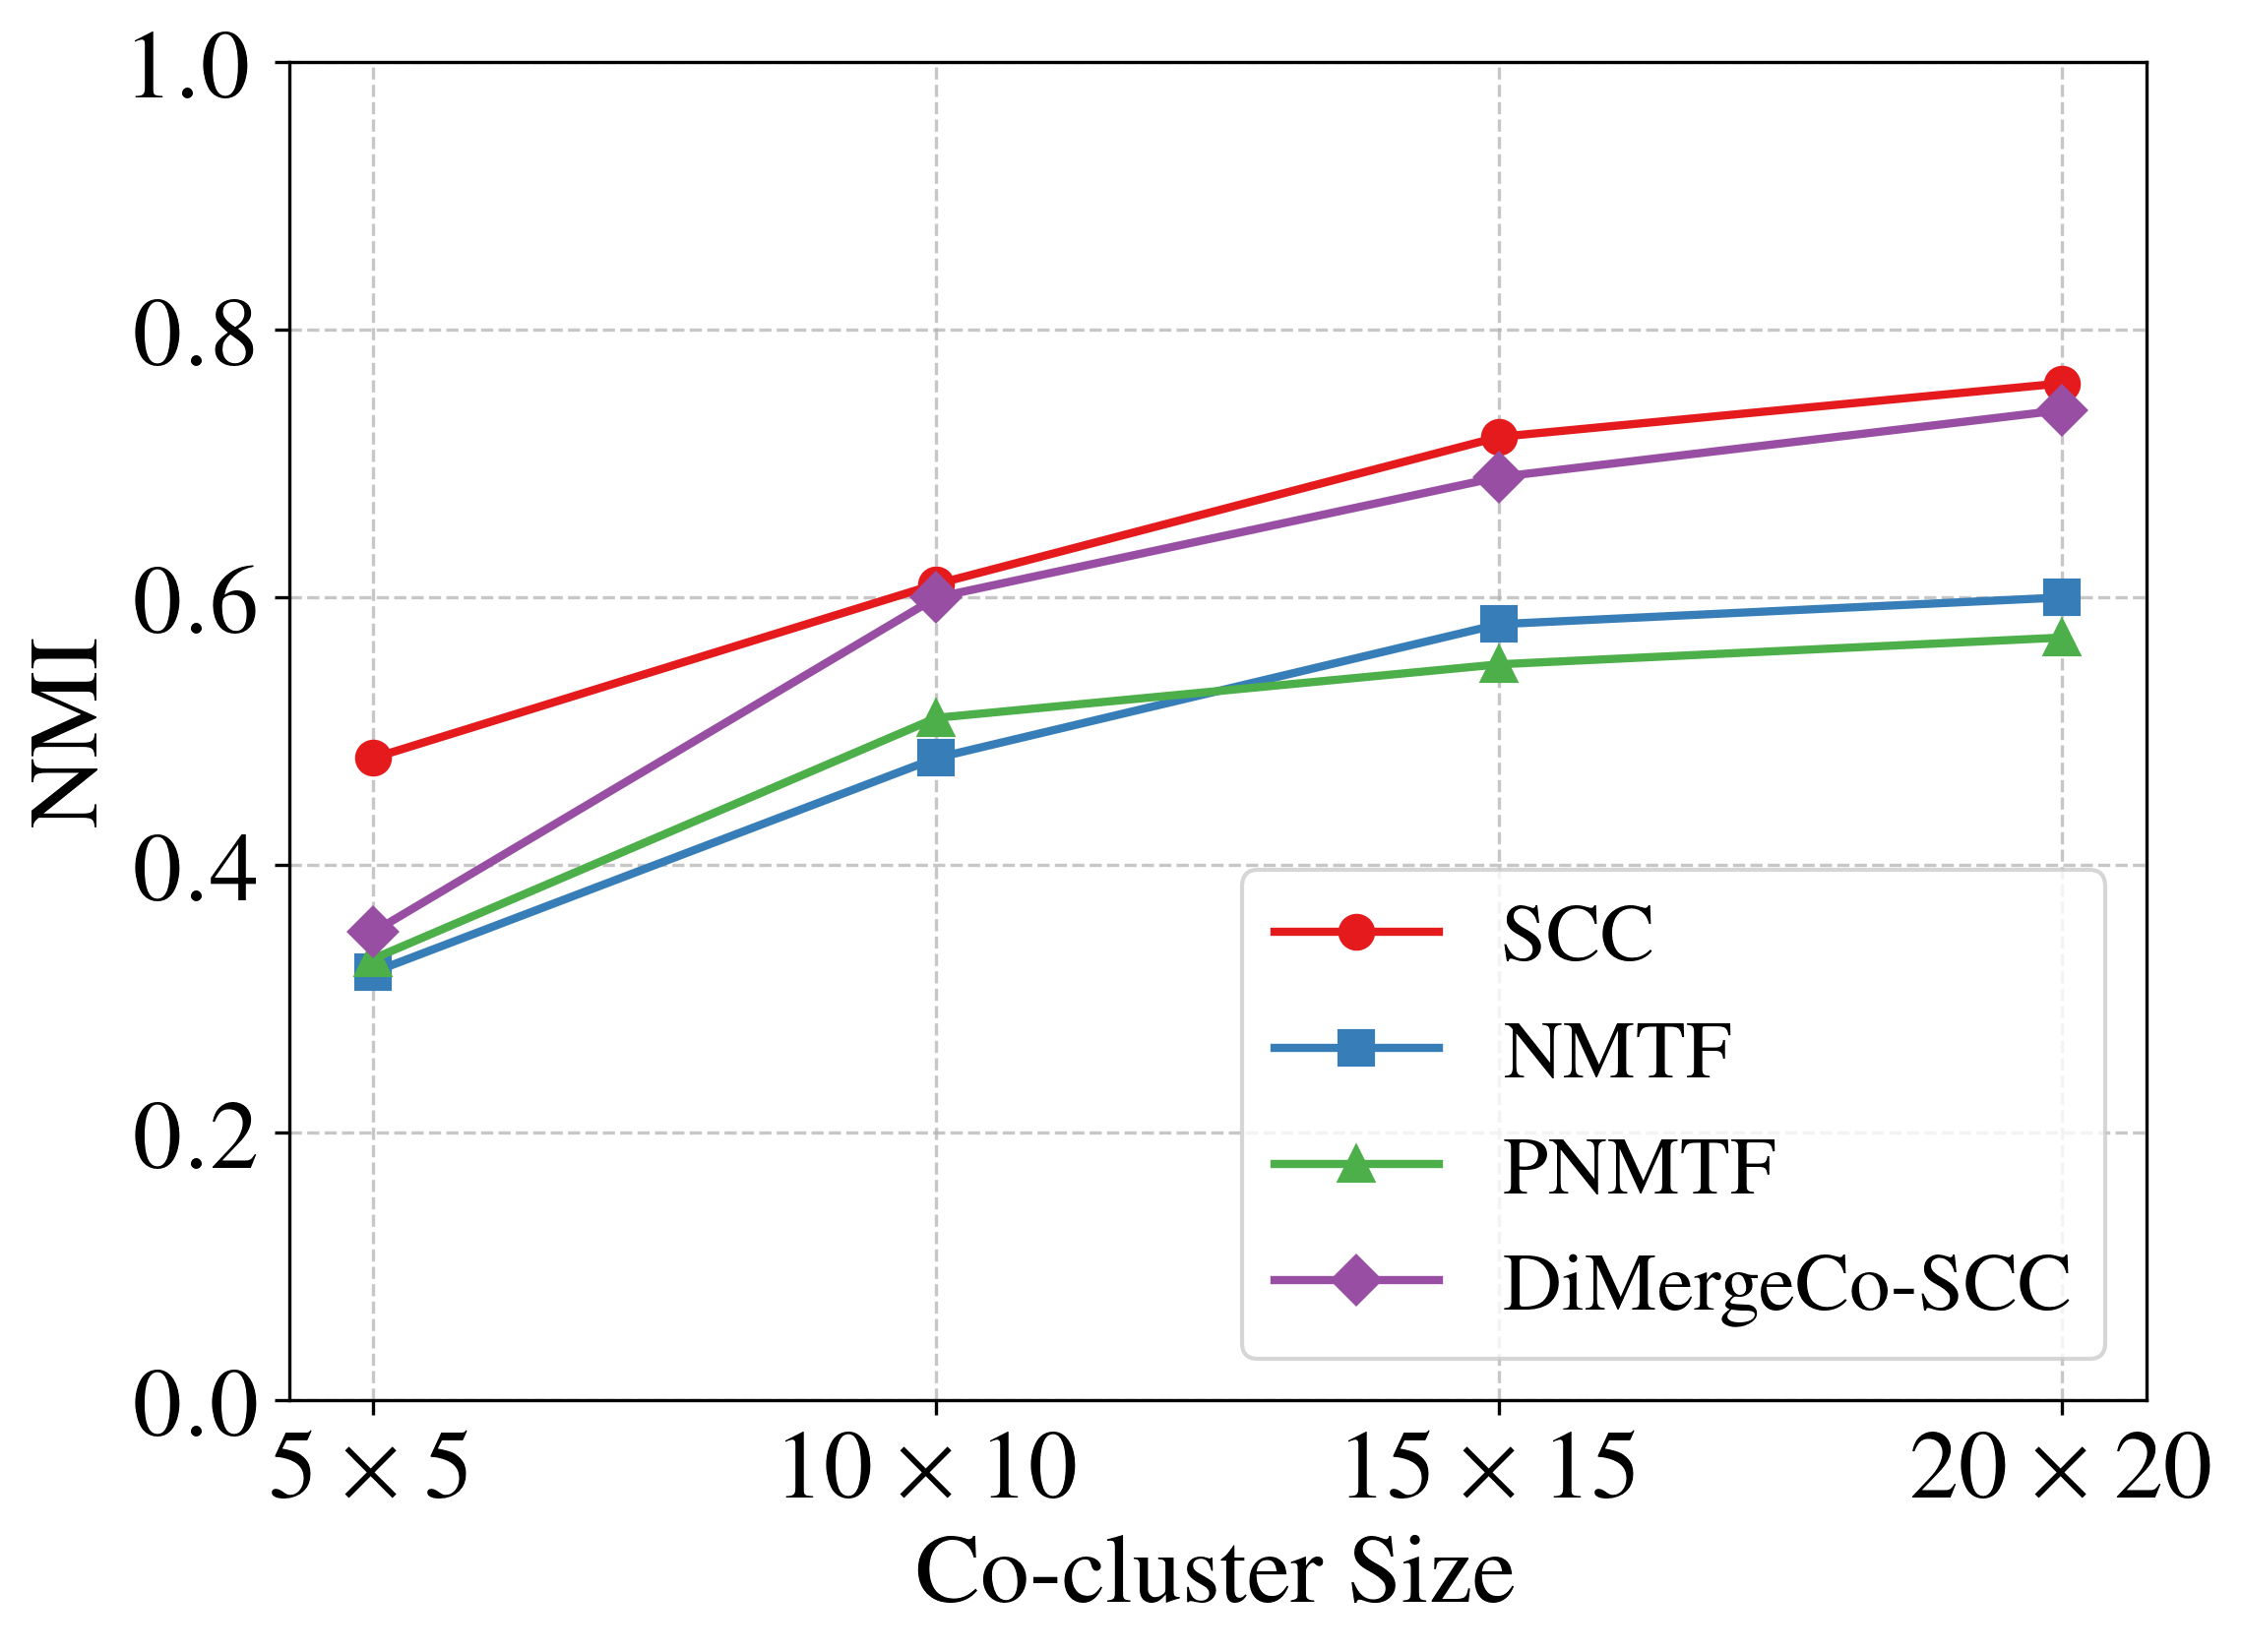
\includegraphics[width=\linewidth]{images/nmi_small.png}
        \caption{NMI for small co-clusters}
        \label{fig:nmi_small}
    \end{subfigure}
    \hfill
    \begin{subfigure}[b]{0.48\textwidth}
        \centering
        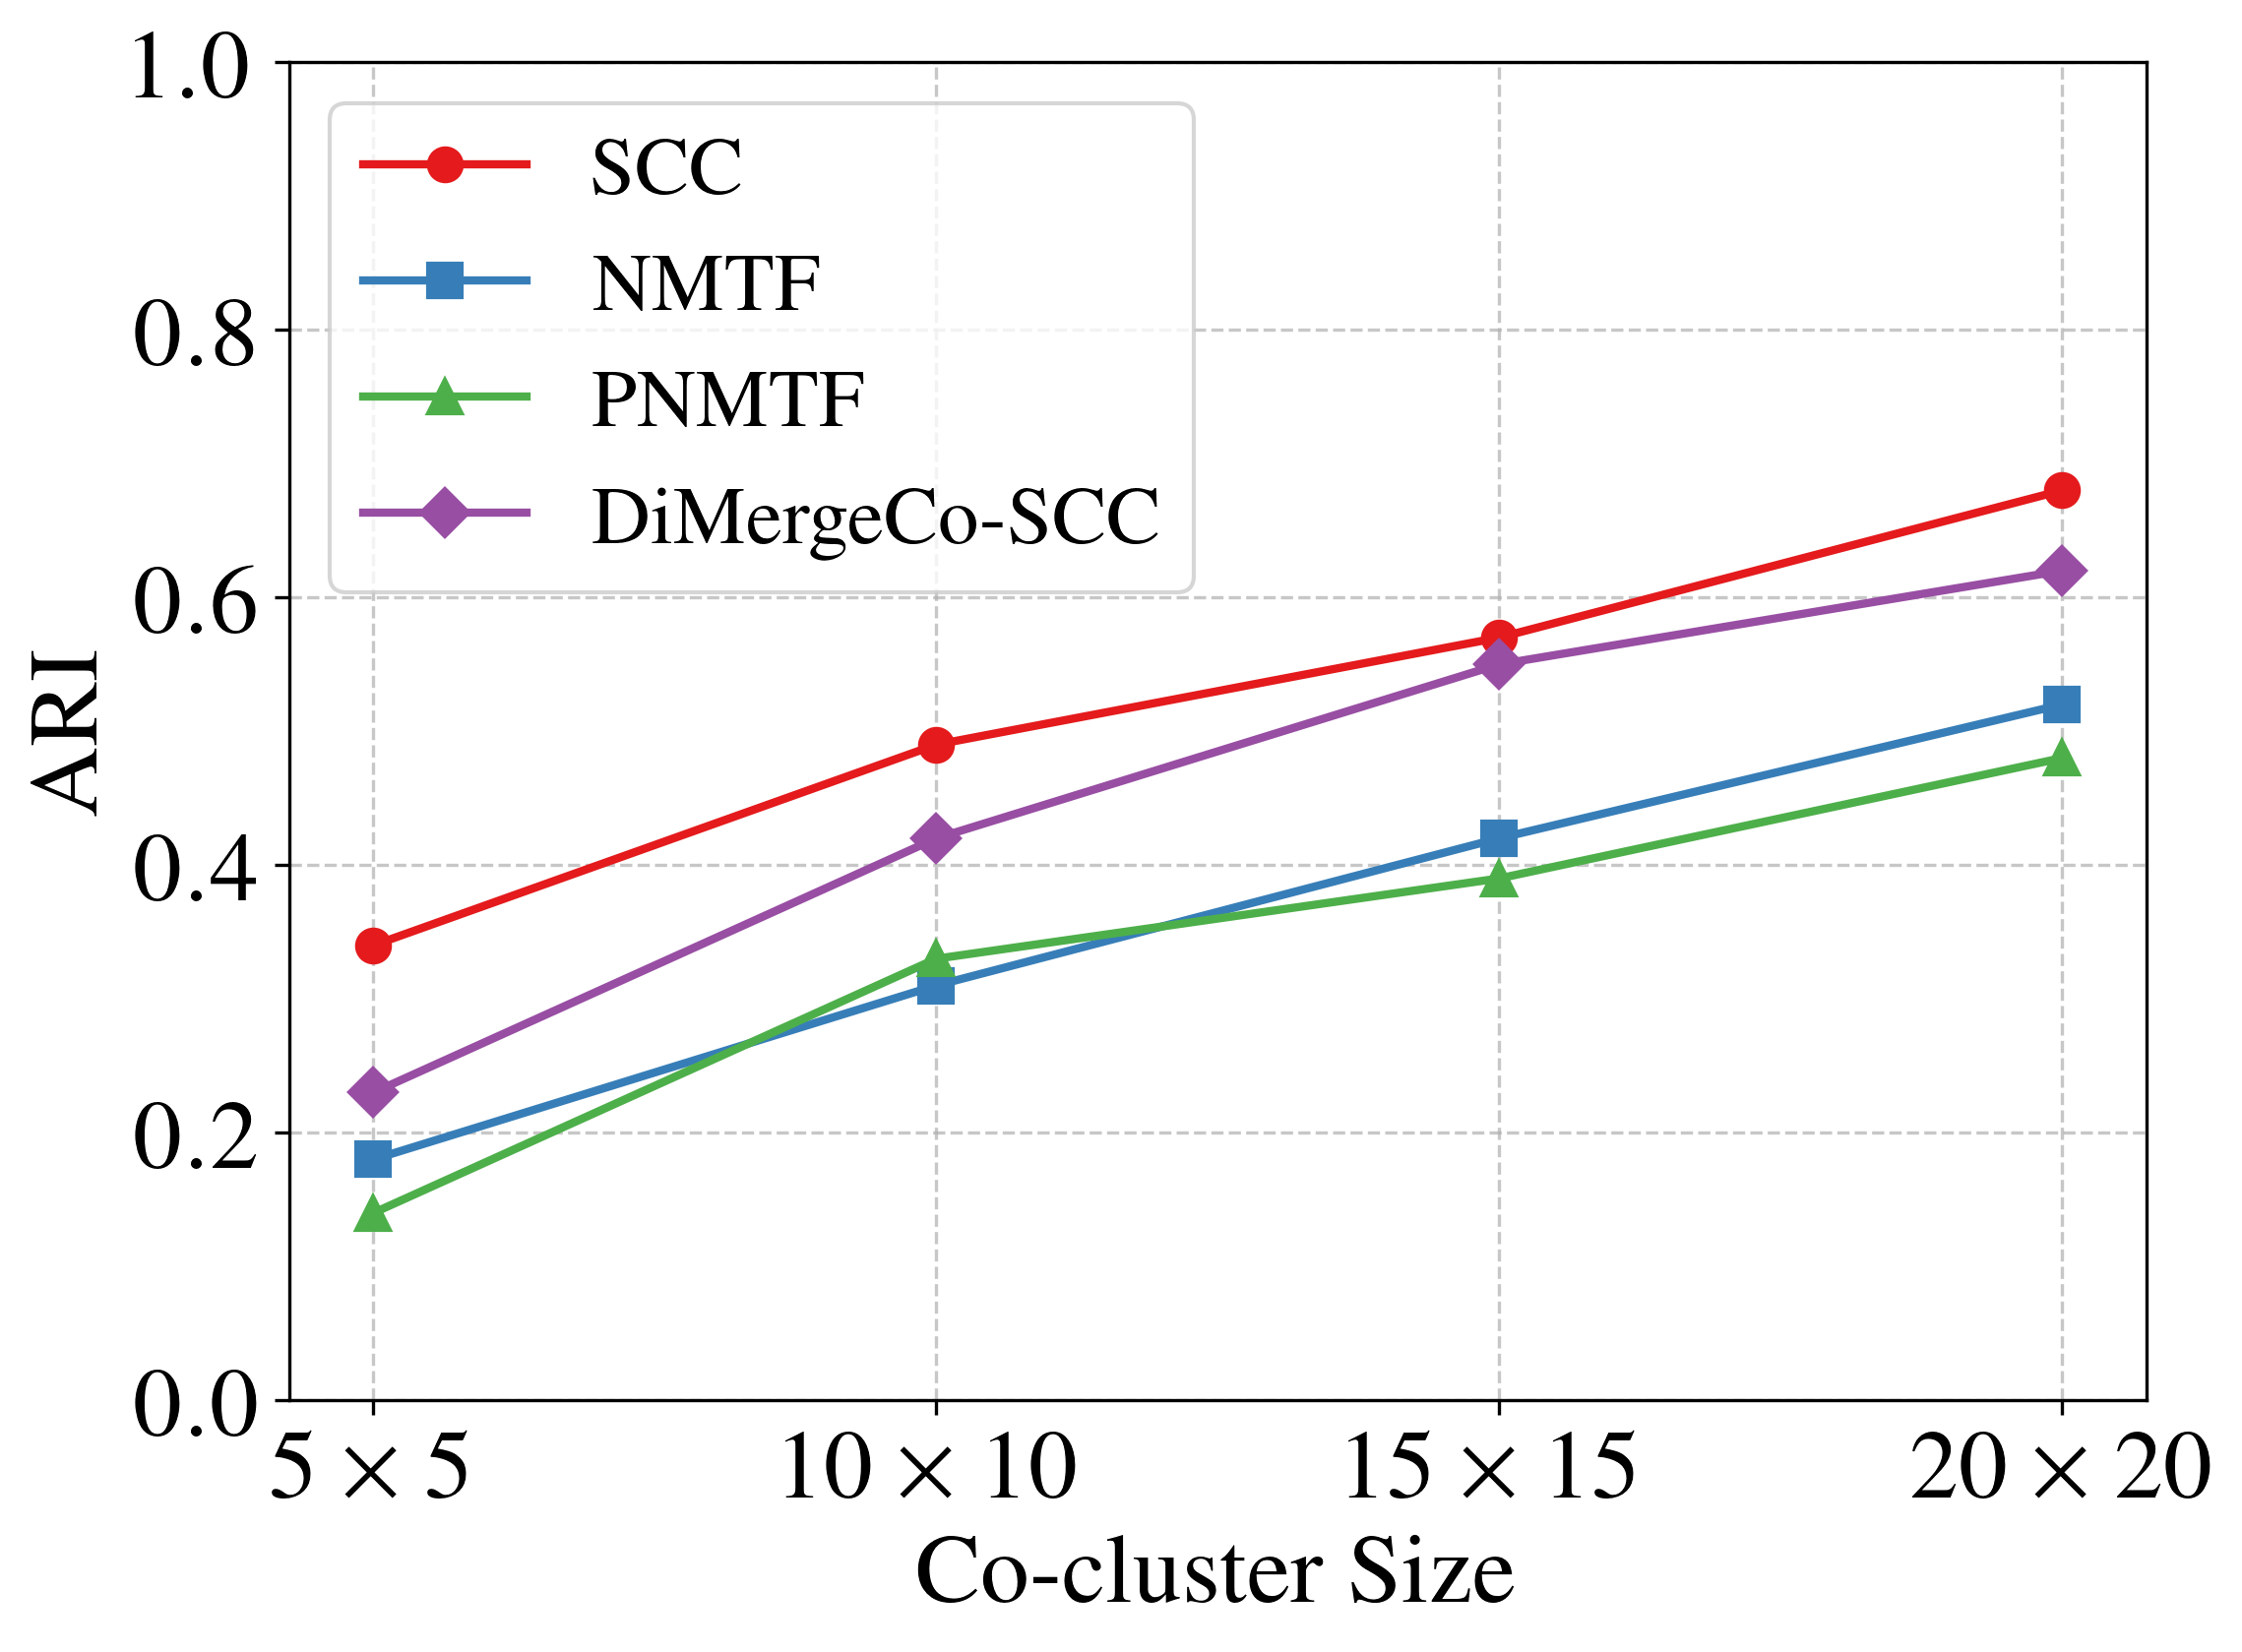
\includegraphics[width=\linewidth]{images/ari_small.png}
        \caption{ARI for small co-clusters}
        \label{fig:ari_small}
    \end{subfigure}
    \caption{Small co-cluster detection results. (a) NMI and (b) ARI performance across different sizes.}
    \label{fig:small-co-cluster-detection}
\end{figure*}

\subsubsection{Clustering Quality Comparison}
\label{subsec:clustering-quality}
Our experimental evaluation compares different co-clustering methods using NMI and ARI metrics (\Cref{tab:evaluation-metrics}). DiMergeCo-SCC achieves superior performance across all datasets, with the highest scores on CLASSIC4 (NMI: 0.8650, ARI: 0.7763), RCV1-Large (NMI: 0.8349, ARI: 0.7576), and Amazon (NMI: 0.7676, ARI: 0.5845). Particularly impressive is its performance on the BCW dataset (NMI: 0.8237, ARI: 0.7403), significantly outperforming PNMTF and ONMTF. This success stems from our probabilistic partitioning strategy and hierarchical merging process, which effectively preserve gene regulatory modules and reconstruct meaningful gene-sample associations. The method's computational efficiency (847.5 seconds) and ability to handle high-dimensional data (11,731 genes, 130 samples) make it particularly valuable for genomics applications.

\subsubsection{Small Co-cluster Detection Analysis}
{\color{blue}
    To validate small co-cluster preservation, we conducted controlled experiments on synthetic $5000 \times 5000$ matrices with planted co-clusters ranging from $5 \times 5$ to $20 \times 20$ with minimum thresholds $T_m = T_n = 5$. As demonstrated in~\Cref{fig:small-co-cluster-detection}, DiMergeCo-SCC consistently outperforms NMTF and PNMTF across all co-cluster sizes, confirming that the proposed multi-sampling, adaptive sizing, and merging mechanisms effectively protect small co-clusters from fragmentation. Notably, for $20 \times 20$ co-clusters, it achieves NMI=0.74 and ARI=0.62, closely matching SCC's performance (NMI=0.76, ARI=0.68) while offering distributed processing capabilities that SCC lacks. This empirically validates our theoretical guarantees and supports DiMergeCo's applicability to real-world datasets where small co-clusters are common.
}

\subsection{Scalability Analysis}
\label{subsec:scalability-analysis}
To evaluate the efficiency of our proposed co-clustering method, we conducted experiments varying the number of processing nodes. The datasets used for this evaluation included Amazon 1000\cite{ni2019JustifyingRecommendationsUsing}, CLASSIC4, and RCV1-Large\cite{lewis2004Rcv1NewBenchmark}. Each dataset was subjected to co-clustering using 1, 4, 8, 16, and 24 processing nodes. {\color{blue}The efficiency metric is defined as $E(P) = S(P)/P = T_1/(P \times T_P)$, where $T_1$ is the execution time on a single node, $T_P$ is the execution time on $P$ nodes, and $S(P)$ is the speedup factor. For clarity, $E(1) = 1$ for a single node.} The results, plotted in~\Cref{fig:efficiency}, demonstrate the efficiency improvements achieved by leveraging parallel processing.

% include images/efficiency.jpg
\begin{figure}[htbp]
    \centering
    
\includegraphics[width=0.8\linewidth]{efficiency.png}
    \caption{Enhanced efficiency of the proposed method in handling large-scale datasets.}
    \label{fig:efficiency}
\end{figure}

\Cref{fig:efficiency} presents the efficiency of our proposed co-clustering method across different datasets as the number of nodes increases. The datasets considered are Amazon 1000, CLASSIC4, and RCV1-Large. The x-axis represents the number of nodes, while the y-axis indicates the efficiency, normalized to the baseline (single node) efficiency of 1.

For Amazon 1000 Dataset, the efficiency starts at 1 for a single node and gradually decreases to 0.39 as the number of nodes increases to 24. The decrease in efficiency is relatively smooth, indicating that our method scales well but exhibits some overhead as more nodes are added. Despite the reduction in efficiency, the method maintains more than 39\% efficiency with 24 nodes, highlighting the robustness of the algorithm even at higher parallelization levels.

For CLASSIC4 Dataset, the efficiency for CLASSIC4 begins at 1 and decreases to 0.52 with 24 nodes. The drop in efficiency is more pronounced compared to the Amazon 1000 dataset, especially between 4 and 8 nodes, indicating a higher overhead for this dataset as the number of nodes increases. The method still retains more than half of the efficiency at 24 nodes, demonstrating good scalability.

For RCV1-Large Dataset, starting from an efficiency of 1, it decreases to 0.47 at 24 nodes. The decrease is relatively smooth, similar to the Amazon 1000 dataset, but with a slightly steeper decline. The method shows significant efficiency retention at higher node counts, indicating effective parallelization.

\begin{table*}[t]
    \centering
    \caption{Sensitivity of DiMergeCo-SCC to key hyper-parameters (CLASSIC4 dataset). Each size threshold ($T_m=T_n$) was tested against all probability thresholds. Quality is stable for $m\times n\ge64$, while the best trade-off between accuracy and runtime is achieved with $T_m=T_n=20$, $P_{\text{thresh}}=0.95$, and 100 blocks.}
    \label{tab:param_sens}
    \begin{threeparttable}
        \begin{tabular}{cccccccccccccc}
            \toprule
                                &                     & \multicolumn{3}{c}{\textbf{25 blocks}} & \multicolumn{3}{c}{\textbf{64 blocks}} & \multicolumn{3}{c}{\textbf{100 blocks}} & \multicolumn{3}{c}{\textbf{144 blocks}}                                                                                                  \\
            \cmidrule(lr){3-5}\cmidrule(lr){6-8}\cmidrule(lr){9-11}\cmidrule(lr){12-14}
            $T_m{=}T_n$         & $P_{\text{thresh}}$ & NMI                                    & ARI                                    & Time (s)                                & NMI                                     & ARI   & Time (s) & NMI            & ARI            & Time (s)       & NMI   & ARI   & Time (s) \\
            \midrule
            \multirow{3}{*}{10} & 0.90                & 0.742                                  & 0.556                                  & 8,234                                   & 0.758                                   & 0.571 & 4,456    & 0.761          & 0.574          & 3,892          & 0.753 & 0.567 & 4,128    \\
                                & 0.95                & 0.744                                  & 0.558                                  & 9,156                                   & 0.761                                   & 0.574 & 5,123    & 0.764          & 0.577          & 4,567          & 0.756 & 0.570 & 4,892    \\
                                & 0.99                & 0.746                                  & 0.560                                  & 11,890                                  & 0.763                                   & 0.576 & 6,789    & 0.766          & 0.579          & 6,234          & 0.758 & 0.572 & 6,567    \\
            \midrule
            \multirow{3}{*}{20} & 0.90                & 0.751                                  & 0.564                                  & 7,892                                   & 0.768                                   & 0.581 & 3,967    & 0.773          & 0.587          & 3,456          & 0.764 & 0.579 & 3,789    \\
                                & 0.95                & 0.754                                  & 0.567                                  & 8,234                                   & 0.771                                   & 0.584 & 4,123    & \textbf{0.776} & \textbf{0.590} & \textbf{3,628} & 0.767 & 0.582 & 3,892    \\
                                & 0.99                & 0.756                                  & 0.569                                  & 9,567                                   & 0.773                                   & 0.586 & 4,789    & 0.778          & 0.592          & 4,234          & 0.769 & 0.584 & 4,456    \\
            \midrule
            \multirow{3}{*}{30} & 0.90                & 0.728                                  & 0.541                                  & 7,456                                   & 0.745                                   & 0.558 & 3,789    & 0.748          & 0.561          & 3,234          & 0.742 & 0.555 & 3,567    \\
                                & 0.95                & 0.731                                  & 0.544                                  & 7,789                                   & 0.748                                   & 0.561 & 3,892    & 0.751          & 0.564          & 3,345          & 0.745 & 0.558 & 3,678    \\
                                & 0.99                & 0.733                                  & 0.546                                  & 8,567                                   & 0.750                                   & 0.563 & 4,234    & 0.753          & 0.566          & 3,789          & 0.747 & 0.560 & 4,123    \\
            \bottomrule
        \end{tabular}
    \end{threeparttable}
\end{table*}

{\color{blue}
\subsection{Parameter Sensitivity Analysis}
\label{subsec:param-sensitivity}

To evaluate the influence of key parameters on both clustering quality and computational efficiency, we conducted a detailed ablation study on the \textbf{CLASSIC4} dataset. Specifically, we examined the effects of three parameters: (i) the number of blocks in the layout, with square configurations $m \times n \in \{25, 64, 100, 144\}$; (ii) the minimum co-cluster size thresholds, $T_m = T_n \in \{10, 20, 30\}$; and (iii) the detection probability threshold, $P_{\text{thresh}} \in \{0.90, 0.95, 0.99\}$. Each configuration was evaluated using Normalized Mutual Information (NMI), Adjusted Rand Index (ARI), and wall-clock runtime. All reported results are averaged over three independent runs for consistency.

\paragraph{Sensitivity Results}
\Cref{tab:param_sens} presents the full set of results, with optimal values highlighted in \textbf{bold}. Our analysis shows that the minimum co-cluster size threshold has the most significant effect on clustering quality. A low threshold ($T_m = T_n = 10$) leads to the formation of noisy and irrelevant micro-clusters, resulting in degraded performance (NMI $\approx$ 0.746--0.766). Conversely, a high threshold ($T_m = T_n = 30$) filters out too many valid small co-clusters, leading to under-segmentation and reduced accuracy (NMI $\approx$ 0.733--0.753). The intermediate value ($T_m = T_n = 20$) offers the best trade-off, consistently achieving superior performance (NMI $\approx$ 0.756--0.778) by balancing noise suppression with structure preservation.

The block configuration primarily affects runtime rather than clustering quality. With only 25 blocks, limited parallelism causes prolonged runtimes (7,456--11,890 seconds). Increasing the number of blocks to 100 significantly reduces runtime (3,234--6,234 seconds) by improving parallel efficiency without substantial communication overhead. However, further increasing to 144 blocks results in higher overhead from inter-block communication, which offsets the parallelization gains and increases the runtime again.

The detection probability threshold, $P_{\text{thresh}}$, has a relatively minor impact on clustering quality but a noticeable effect on runtime. Raising the threshold from 0.90 to 0.99 yields only marginal NMI improvements (typically 0.002--0.005), but incurs a substantial increase in runtime (30--70\%). This suggests that while higher thresholds may slightly enhance reliability, they do so at a disproportionately high computational cost.

\paragraph{Recommendations}
Based on our empirical findings, we propose the following parameter settings for an effective balance between accuracy and efficiency:
\begin{itemize}
    \item \textbf{Block configuration:} Use a square $10 \times 10$ layout (100 blocks), which minimizes runtime without compromising clustering quality.
    \item \textbf{Minimum co-cluster size:} Set $T_m = T_n = 20$ to effectively filter noise while preserving meaningful co-cluster structures, consistently yielding the highest NMI and ARI values.
    \item \textbf{Detection probability threshold:} Use $P_{\text{thresh}} = 0.95$ to achieve strong clustering reliability with a reasonable computational cost. Increasing to 0.99 offers minimal performance gains (less than 0.5\%) at the expense of significantly longer runtimes.
\end{itemize}
}

\section{Conclusion}
\label{sec:conclusion}
We presented DiMergeCo, a scalable co-clustering method for large-scale datasets, leveraging a divide-and-conquer strategy to partition the input matrix into smaller submatrices for parallel processing, thereby significantly reducing computational overhead. Each submatrix is co-clustered independently using a probabilistic model-based optimal partitioning algorithm, ensuring the integrity of co-clusters, and the results are combined using a hierarchical co-cluster merging algorithm to enhance accuracy and reliability. Our implementation using MPI distributes the computational load across multiple nodes, improving scalability and making the approach practical for large-scale applications without requiring specialized performance from any single node. {\color{blue}Experimental results on diverse datasets spanning text documents, recommendation systems, and gene expression data demonstrate substantial improvements in computational efficiency and scalability, confirming the method's effectiveness across different data types and scales.} This work addresses the challenges of co-clustering large-scale data by integrating efficient partitioning, parallel processing, and robust merging techniques, setting a new benchmark for scalable co-clustering and paving the way for future research in scalable data analysis technologies.

\printbibliography
\end{document}
